% =============================================================================
%  Hardness-Aware Robustness of LLM-Text Detection Under Iterative Paraphrasing
%  arXiv preprint format: single column, generous margins, larger figures.
%
%  To convert to ACL 2-column for venue submission later: swap the documentclass
%  block below for the ACL version (commented out at the bottom of this file).
% =============================================================================
\documentclass[11pt,a4paper]{article}

\usepackage[T1]{fontenc}
\usepackage[utf8]{inputenc}
\usepackage[margin=1in]{geometry}
\usepackage{times}
\usepackage{microtype}
\usepackage{textcomp}            % for \textvisiblespace and other glyphs
\usepackage{amsmath,amssymb}
\usepackage{booktabs}
\usepackage{multirow}
\usepackage{graphicx}
\usepackage{xcolor}
\usepackage{url}
\usepackage{hyperref}
\hypersetup{colorlinks=true,linkcolor=blue!50!black,
            citecolor=blue!50!black,urlcolor=blue!50!black}
\usepackage[round,authoryear]{natbib}
\usepackage{titlesec}
\titleformat*{\section}{\large\bfseries}
\titleformat*{\subsection}{\normalsize\bfseries}
\usepackage[section]{placeins}   % keeps floats within their own section
\usepackage{subcaption}          % for side-by-side figures
\usepackage{float}               % provides [H] placement specifier

% ── Float spacing (slightly tighter than default but room to breathe) ───────
\setlength{\textfloatsep}{12pt plus 2pt minus 4pt}
\setlength{\floatsep}{10pt plus 2pt minus 2pt}
\setlength{\intextsep}{10pt plus 2pt minus 2pt}
\renewcommand{\topfraction}{0.85}
\renewcommand{\bottomfraction}{0.70}
\renewcommand{\textfraction}{0.10}
\renewcommand{\floatpagefraction}{0.80}

\graphicspath{{figures/}{../figures/}}

\title{\textbf{Hardness-Aware Robustness of LLM-Text Detection \\
       Under Iterative Paraphrasing: A Mechanistic Analysis}}

\author{Mohammad Arifur Rahman \\
        Anderson University \\
        \texttt{rahman.arif.cse@gmail.com}}

\date{}

\begin{document}
\maketitle

% =============================================================================
\begin{abstract}
We study the robustness of LLM-text detectors under iterative paraphrasing
attacks, asking how degradation distributes across example hardness, not
just on aggregate. On a balanced 1{,}000-paragraph human-vs-Llama-3.1-8B
benchmark we make four contributions.
\textbf{(1) Hardness-specific collapse.} Under simplified paraphrasing, a
character-$n$-gram TF-IDF detector loses
$\Delta F_1 = -0.587$ in the Hard tertile (readability) after two rounds
(0.923\,$\to$\,0.336); RoBERTa-base loses only $-0.080$.
\textbf{(2) Paraphraser diversity.} The collapse reproduces under three
paraphrasers from distinct model families (Llama-3.1-8B, Mistral-7B,
NLLB-200 back-translation), ruling out a single-model confound.
\textbf{(3) Asymmetric flips.} Failure is pure recall loss: all 16
char-TF-IDF flip cases are LLM texts misclassified as human
(73\% of LLM Hard examples); zero human Hard texts flip.
\textbf{(4) Mechanism.} Exact linear SHAP attribution shows only 13\% of
top features survive; formal academic $n$-grams are replaced by short generic
ones. SBERT embedding analysis confirms the asymmetry: Human/LLM centroid
cosine-distance shrinks 21\% across rounds while char-TF-IDF $F_1$ drops
64\% — the signal persists in deep representations, only the surface
encoding collapses.
We argue that hardness-stratified evaluation, paraphraser diversity, and
flip-level attribution should be standard practice for detection robustness studies.

\end{abstract}

% =============================================================================
\section{Introduction}

Detectors for LLM-generated text are deployed in academic-integrity,
plagiarism, and content-moderation pipelines.
Public benchmarks report high accuracy—95\%+ is routine for fine-tuned
classifiers on in-distribution data—but practitioners observe sharp
degradation once text is paraphrased, even
mildly~\citep{krishna2023paraphrasing,sadasivan2023can}.
Two questions about this degradation remain under-studied:

\begin{enumerate}
\item Does degradation hit all examples equally, or is it concentrated on a
predictable subset?
\item Is it a property of a specific paraphraser/detector pair, or a more
general phenomenon that survives changes of paraphraser family?
\end{enumerate}

This paper takes both questions seriously. We use a hardness-aware evaluation
framework: every test example is assigned an Easy/Medium/Hard tertile
\emph{before} the detector ever sees a paraphrase, using
text-only signals (readability, type-token ratio, length).
We then track per-bucket $F_1$ across iterative paraphrase rounds
(P0 $\to$ P1 $\to$ P2), three detector families
(word/char TF-IDF, RoBERTa-base), three paraphrasers from
distinct families (Llama-3.1-8B, Mistral-7B, NLLB-200), and two paraphrase
styles (\emph{standard}: preserve meaning; \emph{simplified}: rewrite in
non-expert style).

\paragraph{Contributions.}
\begin{enumerate}
\item A \textbf{hardness-aware robustness curve}
(\S\ref{sec:hardness}) localising the collapse to the Hard tertile —
Easy and Medium examples are largely unaffected.
\item A \textbf{detector-family asymmetry}
(\S\ref{sec:detector_family}): char-TF-IDF collapses, word-TF-IDF degrades
modestly, RoBERTa-base barely moves.
\item A \textbf{paraphraser-diversity ablation}
(\S\ref{sec:paraphraser_diversity}) reproducing the collapse under Mistral-7B
and NLLB-200 back-translation.
\item A \textbf{mechanistic flip analysis} (\S\ref{sec:mechanism}) tracing
the collapse to surface-feature erosion (13\% feature survival,
formal $\to$ generic $n$-grams, vocabulary homogenisation) and showing all
flips are pure recall loss.
\end{enumerate}

A secondary contribution (\S\ref{sec:calibration}) is that
\textbf{calibration} of TF-IDF detectors does not survive distribution
shift: a temperature fit on the validation set lowers ECE at P0 but
\emph{increases} it at P2-simplified by ${\sim}0.12$, while RoBERTa's
miscalibration is large but stable across stages.

% =============================================================================
\section{Related Work}

\paragraph{LLM-text detection.}
Early detectors used surface statistics
(GLTR~\citep{gehrmann2019gltr}, log-perplexity); contemporary
systems either fine-tune large transformer encoders
(e.g.\ RoBERTa with synthetic LLM data~\citep{guo2023gpt}),
use zero-shot perturbation methods
(DetectGPT~\citep{mitchell2023detectgpt}),
or watermark-based detection~\citep{kirchenbauer2023watermark}.
TF-IDF $+$ logistic regression remains a competitive shallow baseline and is
the most commonly deployed system in production-style settings.

\paragraph{Paraphrasing as attack.}
\citet{krishna2023paraphrasing} introduce DIPPER, a dedicated paraphrase
attacker that breaks GPT-2 watermarking and substantially reduces detector
accuracy. \citet{sadasivan2023can} argue, on theoretical and empirical
grounds, that reliable LLM-text detection may be unattainable in the limit
of paraphrasing. Most empirical work reports degradation as an aggregate
$F_1$ or accuracy drop.

\paragraph{Hardness-stratified evaluation.}
Stratified reporting is standard in machine reading
comprehension~\citep{rajpurkar2018know} and computer vision robustness
benchmarks~\citep{taori2020measuring}, but rare in LLM-text
detection. We argue this is the missing layer of analysis: it pins down
\emph{where} a detector fails, which is a prerequisite for mechanistic explanation.

% =============================================================================
\section{Experimental Setup}
\label{sec:setup}

\subsection{Data}
We use 1{,}000 short paragraphs (100--200 words):
500 human-written (extracted from Wikipedia featured-article paragraphs)
and 500 generated by Llama-3.1-8B-Instruct.
A fixed 80/10/10 split gives 800 train / 100 val / 100 test paragraphs,
balanced by class within each split.
This benchmark deliberately keeps the test set small so we can run multiple
paraphrasers exhaustively; we report 95\% CIs throughout.

\subsection{Paraphrasing tracks}
Each test paragraph is paraphrased twice in sequence, producing P1 (one
paraphrase) and P2 (a paraphrase of P1). We use two prompt styles:

\begin{itemize}
\item \textbf{Standard}: \emph{``Paraphrase the paragraph while preserving meaning and factual
content. Output must be ONE paragraph only (no newlines). Keep length between 100 and
200 words. No lists, bullet points, headings, or citations. Keep all key facts; do not
add new facts.''}

\item \textbf{Simplified}: \emph{``Rewrite the paragraph in a simplified, non-expert style
(easy to understand), while preserving meaning and factual content. Output must be ONE
paragraph only. Keep length between 100 and 200 words. Use simple vocabulary and shorter
sentences. Avoid technical jargon unless necessary. No lists, bullet points, headings,
citations. Do not add new facts.''}
\end{itemize}

We run this with three paraphrasers from distinct families:
\textbf{Llama-3.1-8B-Instruct} (Meta), \textbf{Mistral-7B-Instruct}
(Mistral AI), and \textbf{NLLB-200-distilled-600M}~\citep{nllb2022} via
en\,$\to$\,fra\,$\to$\,en back-translation, which uses no LLM at all.

\subsection{Detectors}
\begin{itemize}
\item \textbf{word\_tfidf\_lr}: TF-IDF over word 1--2 grams ($\leq$50K features,
$min\_df=2$) + $\ell_2$ logistic regression.
\item \textbf{char\_tfidf\_lr}: TF-IDF over character 3--5 grams (\texttt{char\_wb}
analyzer, $\leq$100K features, sublinear TF) + LR.
\item \textbf{roberta\_base}: \texttt{roberta-base} fine-tuned for 3 epochs,
batch size 16, lr=$2\!\times\!10^{-5}$, warmup ratio 0.1.
We run 3 seeds (42, 123, 456) and report mean $\pm$ 95\% CI.
\end{itemize}

\subsection{Hardness definitions}
We define example hardness on the \emph{P0 (original) text only}, before any
paraphrasing or scoring, to avoid circularity. We use four definitions, all
independent of the evaluated detector:

\begin{itemize}
\item \textbf{readability\_fk}: Flesch-Kincaid grade level (primary).
\item \textbf{ttr}: type-token ratio.
\item \textbf{length}: character count.
\item \textbf{perplexity\_gpt2}: per-text GPT-2 perplexity. We sort by
$\mathrm{PPL}$ and place the lowest tertile in the Hard bucket — these are
the texts a public, small LM rates as most LM-typical, i.e.\ the texts a
TF-IDF detector ought to be most confident on. They are also predominantly
LLM (median PPL: 11.8 LLM vs.\ 34.0 Human).
\end{itemize}

Each definition partitions the 100 test examples into Easy/Medium/Hard
tertiles ($n \approx 33$ each). Bucket assignments are weakly correlated
across the four signals (pairwise Kendall $\tau$ in $[-0.47, 0.19]$;
Fig.~\ref{fig:concordance}), meaning different examples end up in each
definition's Hard bucket. Nevertheless, the \emph{Hard-bucket $F_1$ collapse
pattern} reproduces under each definition (Fig.~\ref{fig:fig09_multiseed}
and Table~\ref{tab:ppl_collapse}): whatever subset is flagged as Hard, the
relative drop in detector $F_1$ inside that subset is consistent.
We use \texttt{readability\_fk} as the primary stratification because it
has the clearest linguistic interpretation and is stable across runs.

\subsection{Evaluation protocol}
For each (detector, paraphraser, track, round) combination, we report
$F_1$ at the 0.5 threshold, AUROC, AURC (area under the round-by-round
$F_1$ trajectory, Sec.~\ref{sec:robustness}), and ECE.
95\% CIs are paired-bootstrap intervals over 2{,}000 resamples;
multi-seed CIs are reported across $\{42, 123, 456\}$.

% =============================================================================
\section{Aggregate Robustness}
\label{sec:robustness}

We define the \textbf{Area Under the Robustness Curve} (AURC)
\citep[adapted from][]{taori2020measuring} as the mean $F_1$ across rounds
$\{$P0, P1, P2$\}$; a perfectly robust detector has AURC equal to its P0
$F_1$. Table~\ref{tab:aurc} reports standard- and simplified-track AURCs.

\begin{table}[htbp]
\centering
\small
\begin{tabular}{lcc}
\toprule
\textbf{Detector} & \textbf{AURC (standard)} & \textbf{AURC (simplified)} \\
\midrule
char\_tfidf\_lr & 0.874 $\pm$ 0.009 & \textbf{0.649} $\pm$ 0.009 \\
word\_tfidf\_lr & 0.821 $\pm$ 0.011 & \textbf{0.756} $\pm$ 0.011 \\
roberta\_base & 0.849 [0.802, 0.893] & 0.908 [0.867, 0.950] \\
\bottomrule
\end{tabular}
\caption{AURC (mean $F_1$ across P0/P1/P2) by detector and paraphrase style.
Bold = simplified track is substantially worse than standard track.
RoBERTa's standard vs simplified AURCs overlap within their 95\% CIs and we
read the apparent ordering as 3-seed sampling noise rather than a real
effect.
TF-IDF rows: paired-bootstrap 95\% CIs over 20 resamples (LR is deterministic
given a seed). RoBERTa rows: mean $\pm$ 95\% paired-bootstrap CI across 3
random seeds.}
\label{tab:aurc}
\end{table}

Figure~\ref{fig:fig12_three_detector} shows the round-by-round trajectory for
all three detectors. The simplified track collapses char-TF-IDF aggressively
between P0 and P1 and again between P1 and P2; the standard track is nearly
flat for all detectors. \emph{The simplification prompt drives most of the
degradation—not the act of paraphrasing itself.}

\begin{figure}[htbp]
\centering
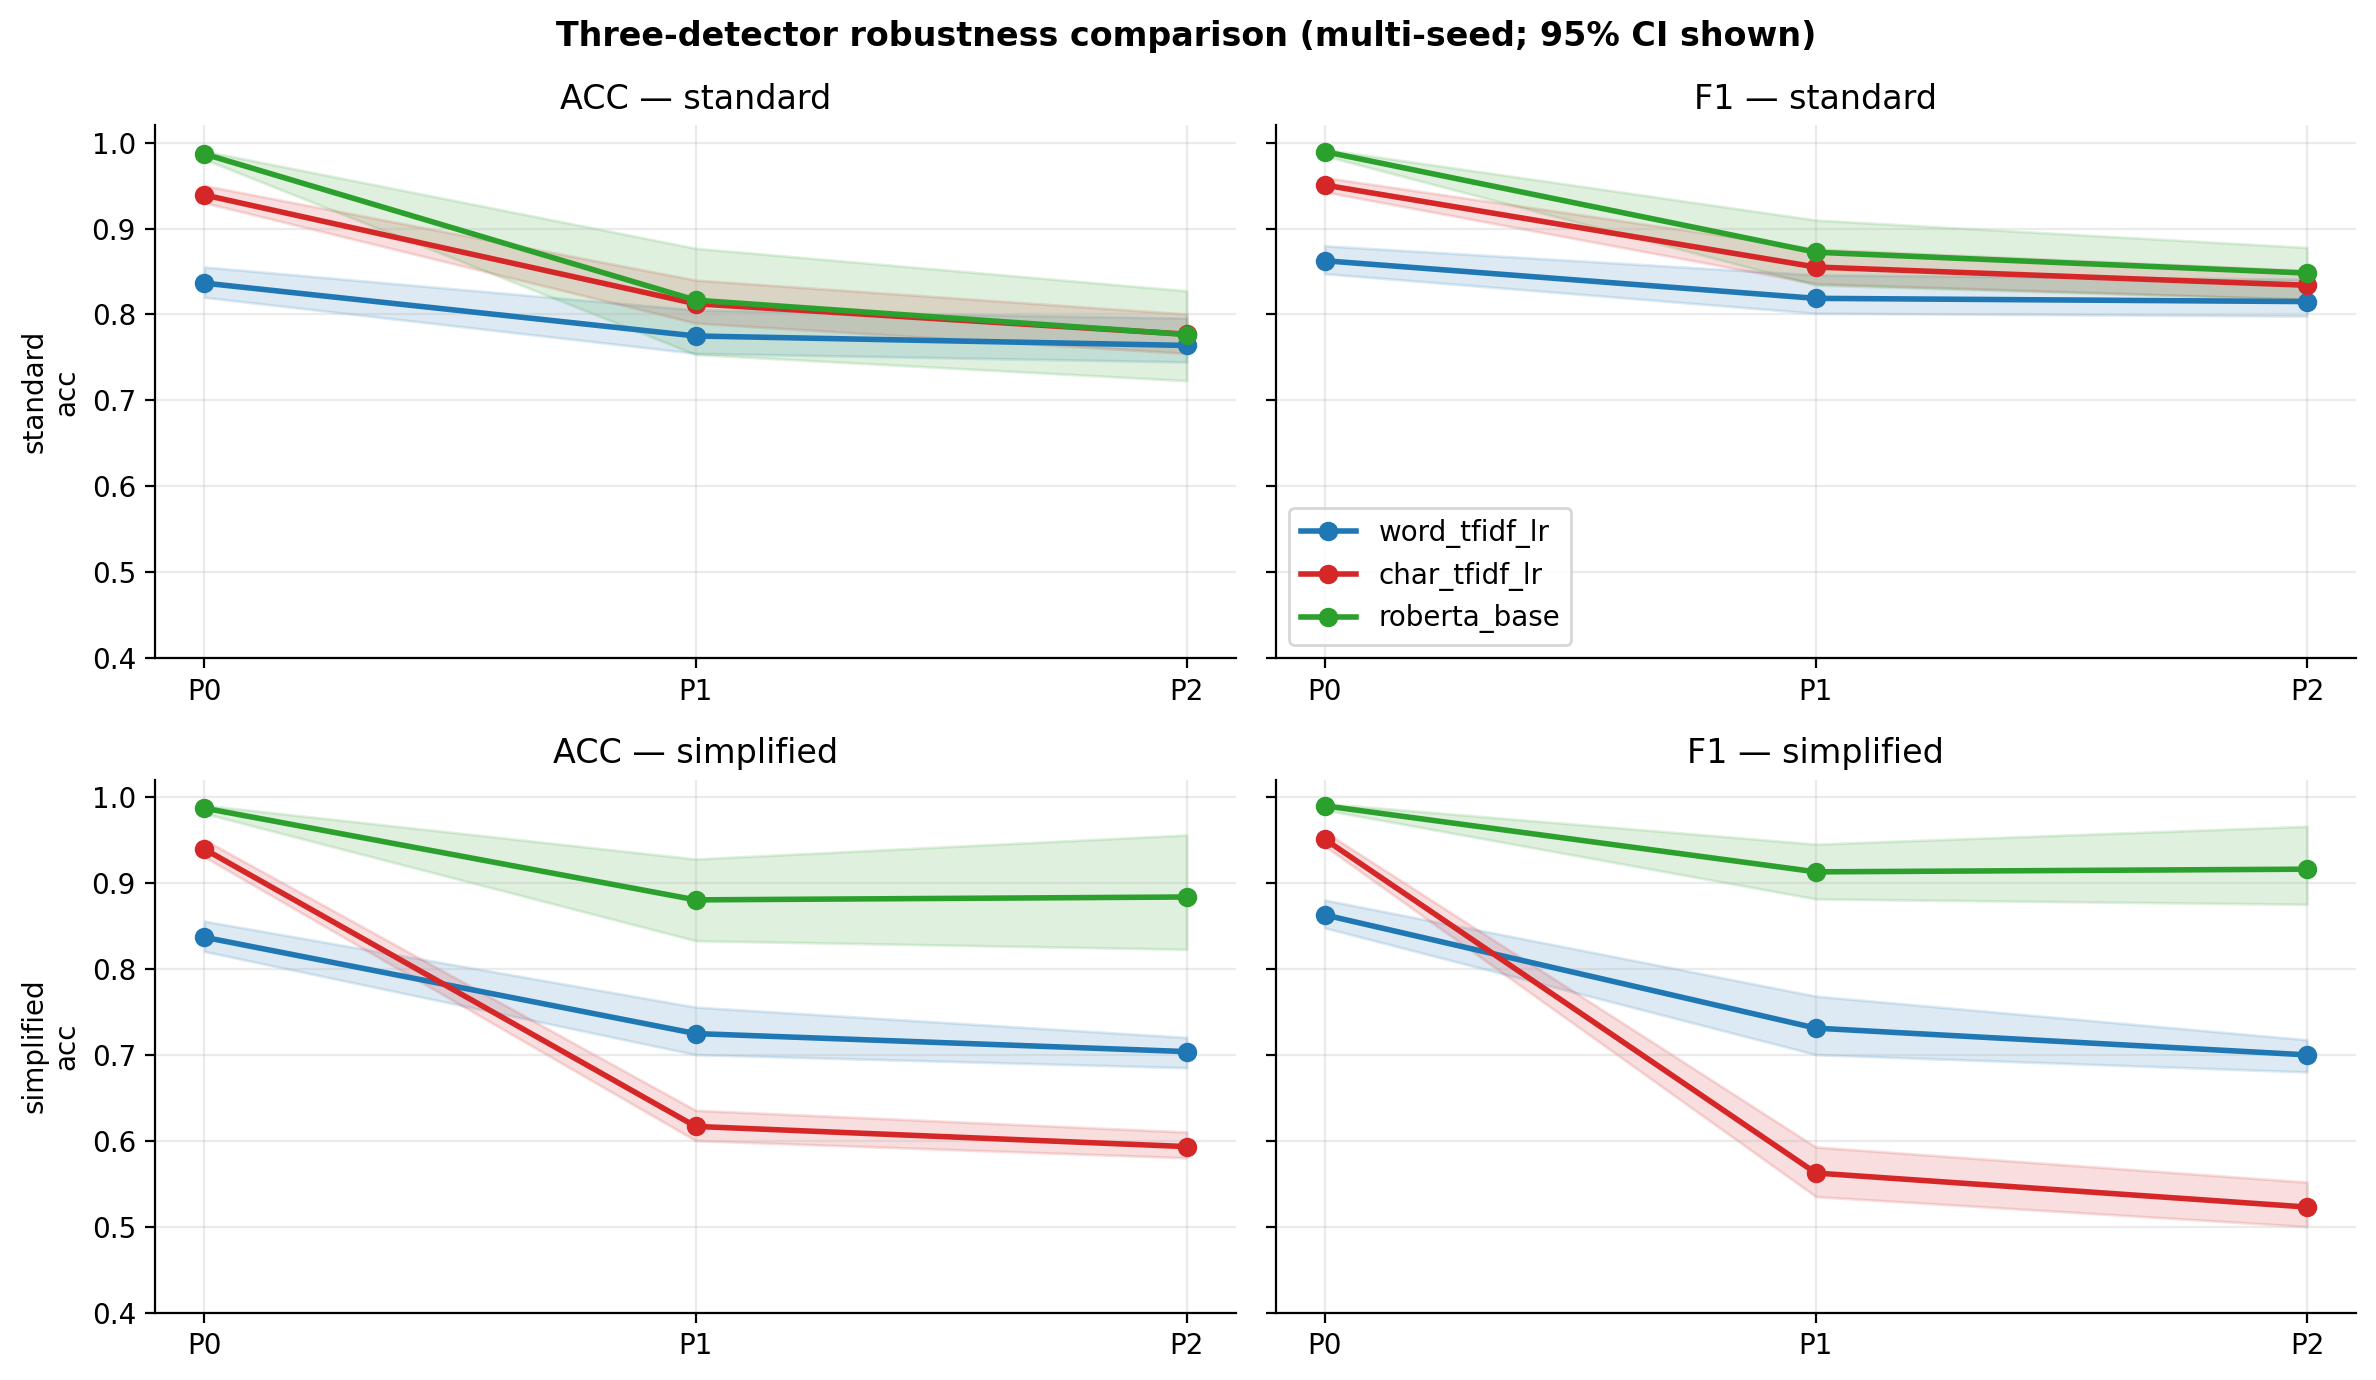
\includegraphics[width=0.82\linewidth]{fig12_three_detector_robustness.png}
\caption{$F_1$ across paraphrase rounds, by detector. The simplified track
collapses char-TF-IDF aggressively; the standard track is essentially flat.
RoBERTa is robust on both.}
\label{fig:fig12_three_detector}
\end{figure}

% =============================================================================
\section{Hardness-Aware Analysis}
\label{sec:hardness}

The headline numbers in Table~\ref{tab:aurc} hide significant heterogeneity.
We now stratify $F_1$ by hardness tertile (readability\_fk on P0 text), and
plot the per-bucket trajectory in Fig.~\ref{fig:fig13_universal}.

\begin{figure}[htbp]
\centering
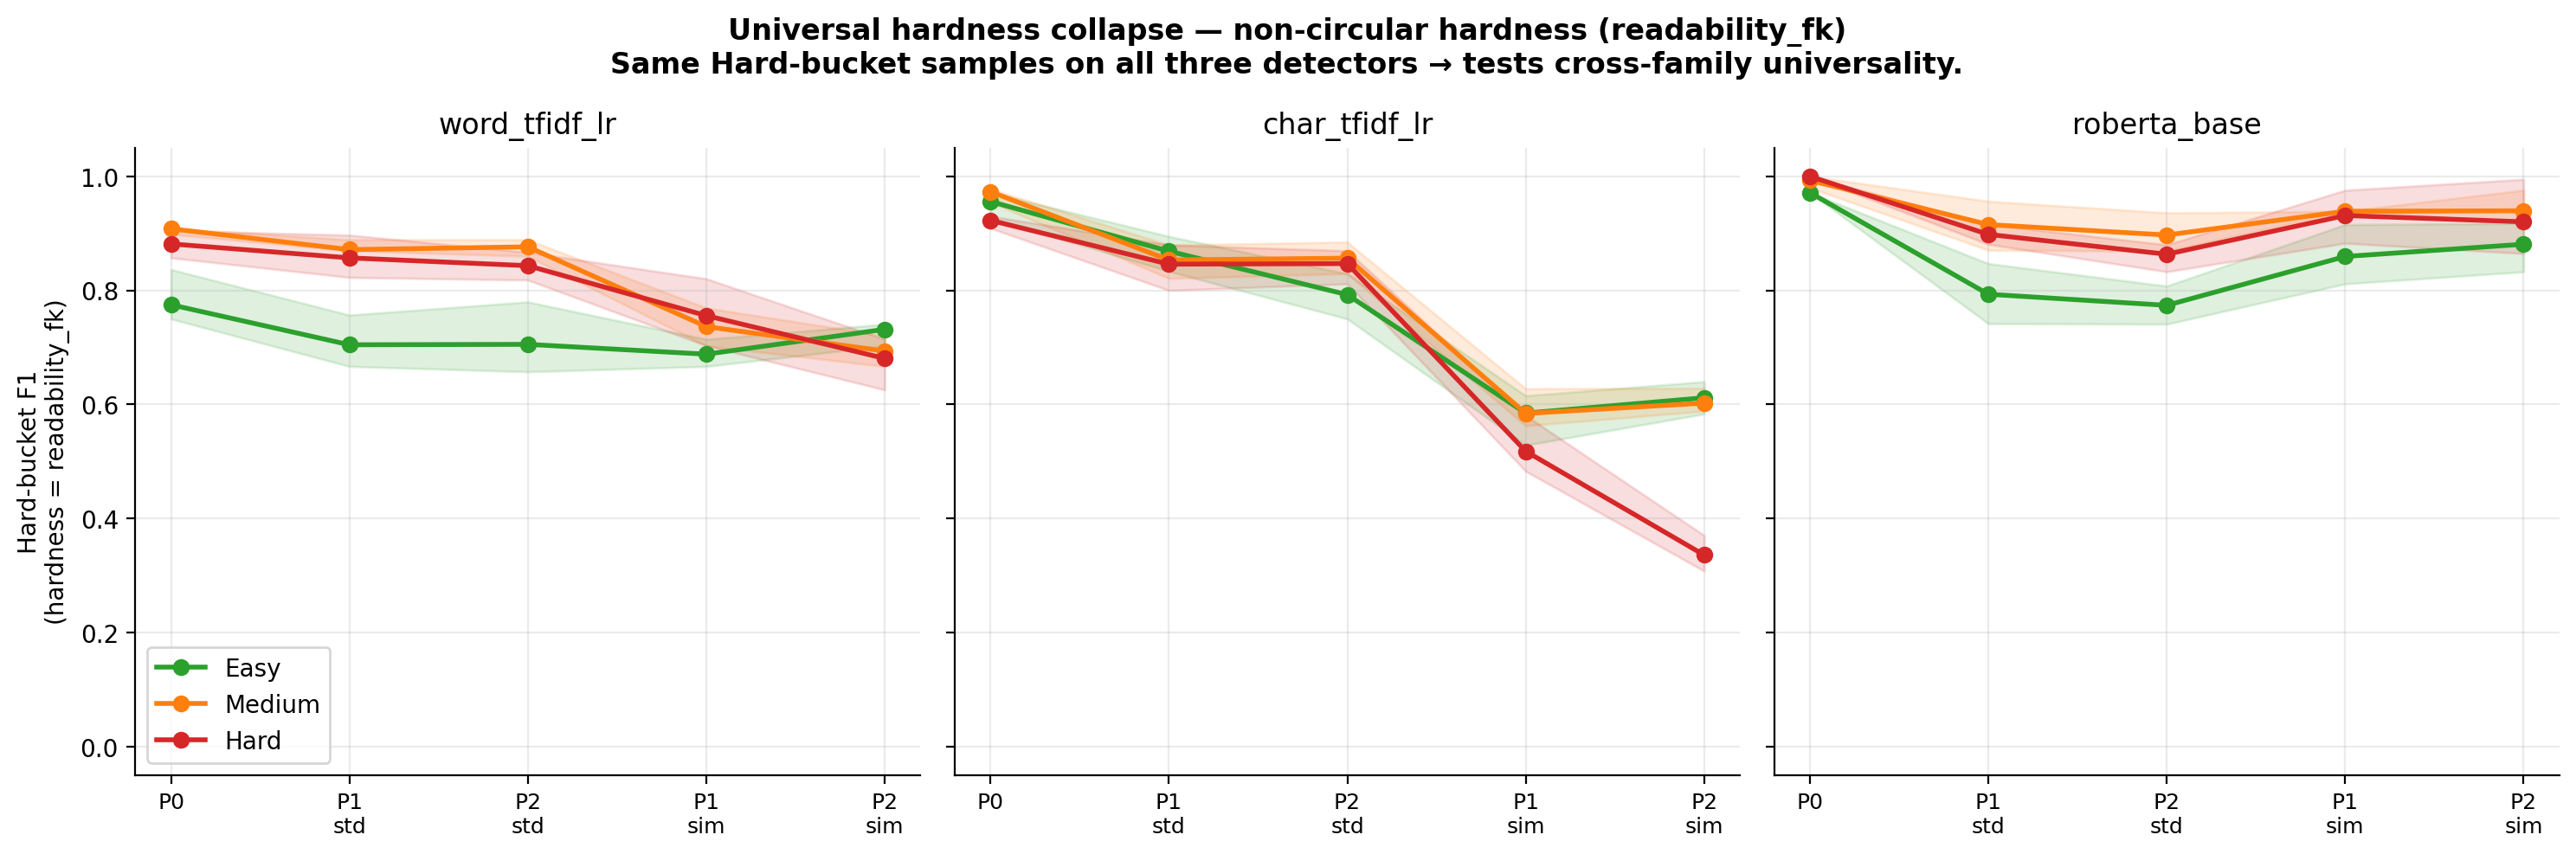
\includegraphics[width=0.82\linewidth]{fig13_universal_hardness_collapse.png}
\caption{Per-tertile $F_1$ trajectory (readability\_fk hardness). The Hard
tertile collapses by $\Delta F_1 \!=\! -0.587$ under simplified paraphrasing for
char-TF-IDF, while Easy/Medium stay above 0.6.}
\label{fig:fig13_universal}
\end{figure}

The Hard tertile (readability\_fk) under the \emph{simplified} track shows the
dominant effect:

\begin{itemize}
\item \textbf{char\_tfidf\_lr}: 0.923 [0.909, 0.930] at P0
       $\to$ 0.336 [0.308, 0.370] at P2.
       This is a \textbf{0.587 drop in $F_1$}, well outside any reasonable CI.
\item \textbf{word\_tfidf\_lr}: 0.882 [0.857, 0.905] at P0
       $\to$ 0.681 [0.626, 0.714] at P2.
       A 0.201 drop—real but smaller.
\item \textbf{roberta\_base}: 1.000 at P0
       $\to$ 0.920 [0.865, 0.995] at P2.
       Only a 0.080 drop — an order of magnitude smaller than char-TF-IDF's
       0.587, and small enough that a single mis-predicted example in a 34-example
       bucket accounts for the entire gap.
\end{itemize}

The Easy and Medium tertiles drop by far less (Fig.~\ref{fig:fig13_universal}).
This is the central empirical claim of the paper: \textbf{simplified paraphrasing
attacks the Hard tail of the test distribution, and surface-feature detectors are
disproportionately exposed.}

\paragraph{Hardness concordance.}
A reader might worry that ``Hard'' is whatever a particular detector finds
hard. We rule this out: hardness is defined from P0 text alone, before the
detector sees a paraphrase. Although the three text-only definitions place
different examples into their Hard buckets (Kendall $\tau$ between $-0.28$ and
$0.13$; Fig.~\ref{fig:concordance}), the Hard-bucket $F_1$ collapse appears
in all three — the detector degrades on whichever subset each definition
flags as Hard (multi-seed grid, Fig.~\ref{fig:fig09_multiseed}).

\paragraph{Robustness to the choice of hardness signal: GPT-2 perplexity.}
Because the three text-only signals are all surface lexical/syntactic
features, a reviewer can reasonably ask whether the collapse is just an
artifact of \emph{lexical formality}. We test this with a fourth, structurally
different hardness signal: per-text perplexity under GPT-2-base. The
``Hard'' bucket here is the low-perplexity tertile — the texts a public LM
considers LM-typical (median 11.8 vs.\ 34.0 for the rest of the test set).
This selects a largely different 34 examples (Kendall $\tau$ vs.\
\texttt{readability\_fk} is $0.13$, p\,$=\,0.13$), yet the collapse
reproduces with comparable magnitude (Table~\ref{tab:ppl_collapse}):
char-TF-IDF $F_1$ drops $0.970 \!\to\! 0.522$ ($\Delta = -0.448$) and
word-TF-IDF $F_1$ drops $0.921 \!\to\! 0.786$ ($\Delta = -0.135$).
The Hard-bucket collapse is therefore not specific to any one definition of
hardness.

\begin{table}[H]
\centering
\small
\begin{tabular}{lccc}
\toprule
\textbf{Detector} & \textbf{P0 Hard $F_1$} & \textbf{P2-sim Hard $F_1$} & $\Delta$ \\
\midrule
\multicolumn{4}{l}{\emph{Hardness = GPT-2 perplexity (low-PPL tertile = Hard)}} \\
char\_tfidf\_lr & 0.970 & 0.522 & $\mathbf{-0.448}$ \\
word\_tfidf\_lr & 0.921 & 0.786 & $-0.135$ \\
\midrule
\multicolumn{4}{l}{\emph{Hardness = readability\_fk (primary, for reference)}} \\
char\_tfidf\_lr & 0.923 & 0.336 & $\mathbf{-0.587}$ \\
word\_tfidf\_lr & 0.882 & 0.681 & $-0.201$ \\
\bottomrule
\end{tabular}
\caption{Hard-bucket $F_1$ under perplexity-based hardness reproduces the
collapse at comparable magnitude to readability-based hardness, despite
selecting a largely different subset of examples (Kendall $\tau = 0.13$ between
the two bucket assignments).}
\label{tab:ppl_collapse}
\end{table}

\begin{figure}[htbp]
\centering
\begin{subfigure}[t]{0.38\linewidth}
  \centering
  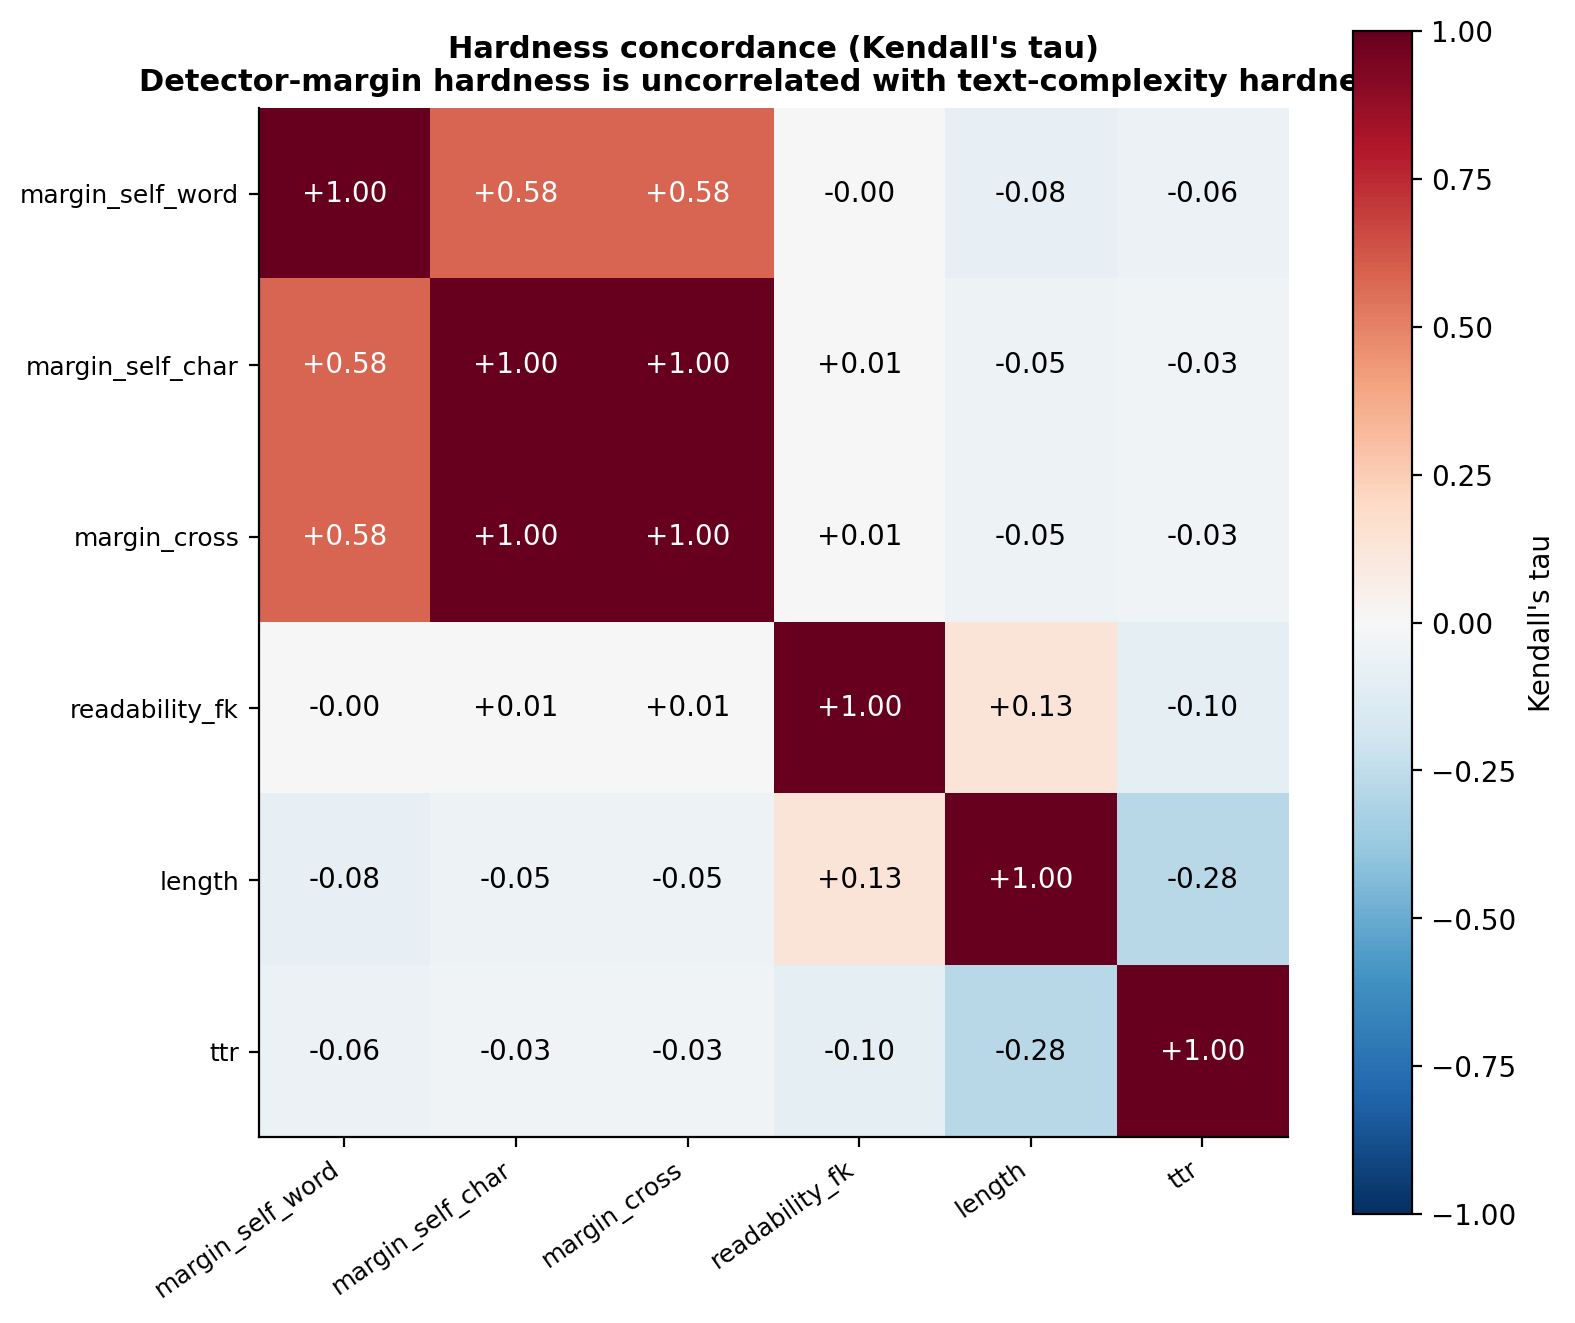
\includegraphics[width=\linewidth]{fig03_hardness_concordance_heatmap.png}
  \caption{Bucket-assignment concordance (Kendall $\tau$) across the three
  text-only definitions (perplexity hardness, added separately, is also
  weakly correlated: $|\tau|\!\le\!0.19$ vs.\ readability/TTR; $\tau\!=\!-0.47$
  vs.\ length, by construction). Bucket assignments diverge, yet the
  collapse reproduces under all four.}
  \label{fig:concordance}
\end{subfigure}
\hfill
\begin{subfigure}[t]{0.58\linewidth}
  \centering
  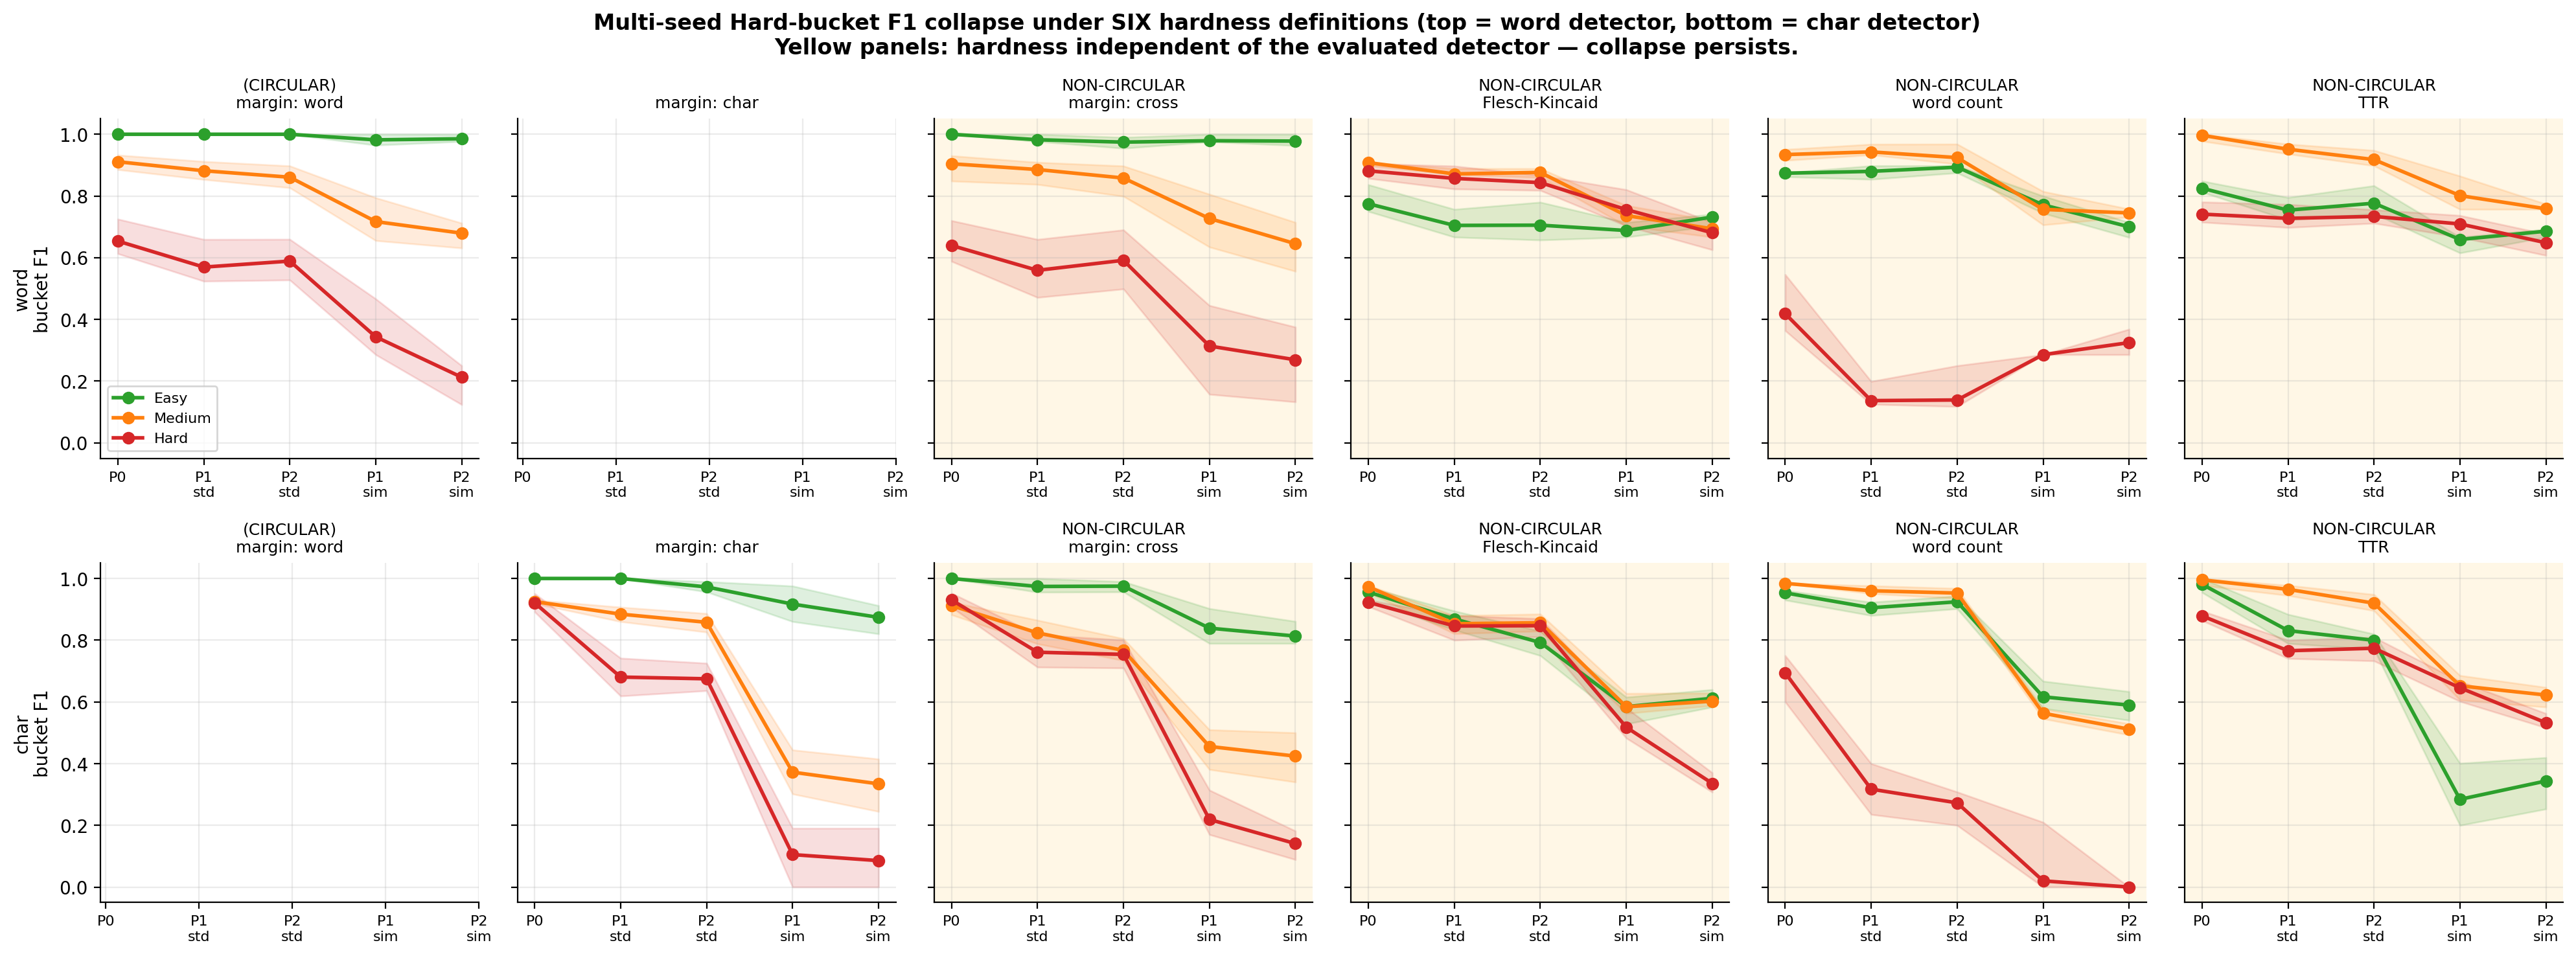
\includegraphics[width=\linewidth]{fig09_multiseed_hardness_grid.png}
  \caption{Multi-seed Hard-tertile $F_1$ (3 seeds, 95\% CI). Collapse
  reproduces under each text-only hardness definition
  (readability\_fk, ttr, length).}
  \label{fig:fig09_multiseed}
\end{subfigure}
\caption{Hardness concordance and multi-seed robustness grid.}
\label{fig:concordance_combined}
\end{figure}

% =============================================================================
\section{Detector-Family Asymmetry}
\label{sec:detector_family}

The three detector families exhibit qualitatively different collapse profiles.
Table~\ref{tab:detector_family} summarises Hard-tertile $F_1$ at the
endpoints. RoBERTa is essentially robust; char-TF-IDF collapses
catastrophically; word-TF-IDF is in between.

\begin{table}[htbp]
\centering
\small
\begin{tabular}{lcccc}
\toprule
\textbf{Detector} & \textbf{Family} & \textbf{P0 Hard $F_1$} & \textbf{P2-sim Hard $F_1$} & \textbf{$\Delta$} \\
\midrule
char\_tfidf\_lr & char $n$-gram & 0.923 & 0.336 & $-0.587$ \\
word\_tfidf\_lr & word $n$-gram & 0.882 & 0.681 & $-0.201$ \\
roberta\_base   & transformer   & 1.000 & 0.920 & $-0.080$ \\
\bottomrule
\end{tabular}
\caption{Hard-tertile $F_1$ collapse by detector family
(readability\_fk hardness, simplified track). Collapse magnitude
scales inversely with the feature granularity: char $\gg$ word $\gg$
contextual.}
\label{tab:detector_family}
\end{table}

We propose a feature-granularity explanation: the simplification prompt
preserves \emph{meaning} (so transformer embeddings are stable) but
destroys \emph{surface form} (so character and word $n$-grams are not).
Section~\ref{sec:mechanism} provides direct evidence for this.

% =============================================================================
\section{Paraphraser Diversity}
\label{sec:paraphraser_diversity}

A natural worry is that the collapse is a property of Llama paraphrasing
specifically (e.g.\ Llama-as-paraphraser may have a systematic style that
Llama-as-generator is unusually vulnerable to). We rule this out by repeating
the simplified-track experiment under two alternative paraphrasers from
unrelated model families:

\begin{itemize}
\item \textbf{Mistral-7B-Instruct} (Mistral AI). Same prompt, different LLM family.
\item \textbf{NLLB-200} en\,$\to$\,fra\,$\to$\,en back-translation. A
multilingual MT system, not an LLM, with no instruction-tuning.
\end{itemize}

Table~\ref{tab:paraphraser_comparison} (visualised in Fig.~\ref{fig:fig17})
shows the Hard-tertile $F_1$ at P2 under each paraphraser. The qualitative
pattern—char-TF-IDF collapses, word-TF-IDF degrades modestly—survives the
change of paraphraser, although the absolute collapse magnitude is largest
under Llama-as-paraphraser.

\begin{table}[htbp]
\centering
\small
\begin{tabular}{lcc}
\toprule
\textbf{Paraphraser} & \textbf{Hard $F_1$ (char)} & \textbf{Hard $F_1$ (word)} \\
\midrule
P0 (no paraphrase)              & 0.923 & 0.882 \\
\midrule
Llama-3.1-8B (simplified)       & \textbf{0.336} & \textbf{0.681} \\
Mistral-7B  (simplified)        & 0.647 & 0.737 \\
Mistral-7B  (standard)          & 0.826 & 0.773 \\
NLLB-200 (en$\to$fr$\to$en)     & 0.483 & 0.703 \\
\bottomrule
\end{tabular}
\caption{Hard-tertile $F_1$ at P2 across four paraphrasers. The collapse
direction is consistent; magnitude is largest for Llama-as-paraphraser on the
simplified track. NLLB-200 (en$\to$fr$\to$en) alone produces a 0.44 drop in
char-TF-IDF Hard $F_1$, ruling out an LLM-only artifact.}
\label{tab:paraphraser_comparison}
\end{table}

\begin{figure}[htbp]
\centering
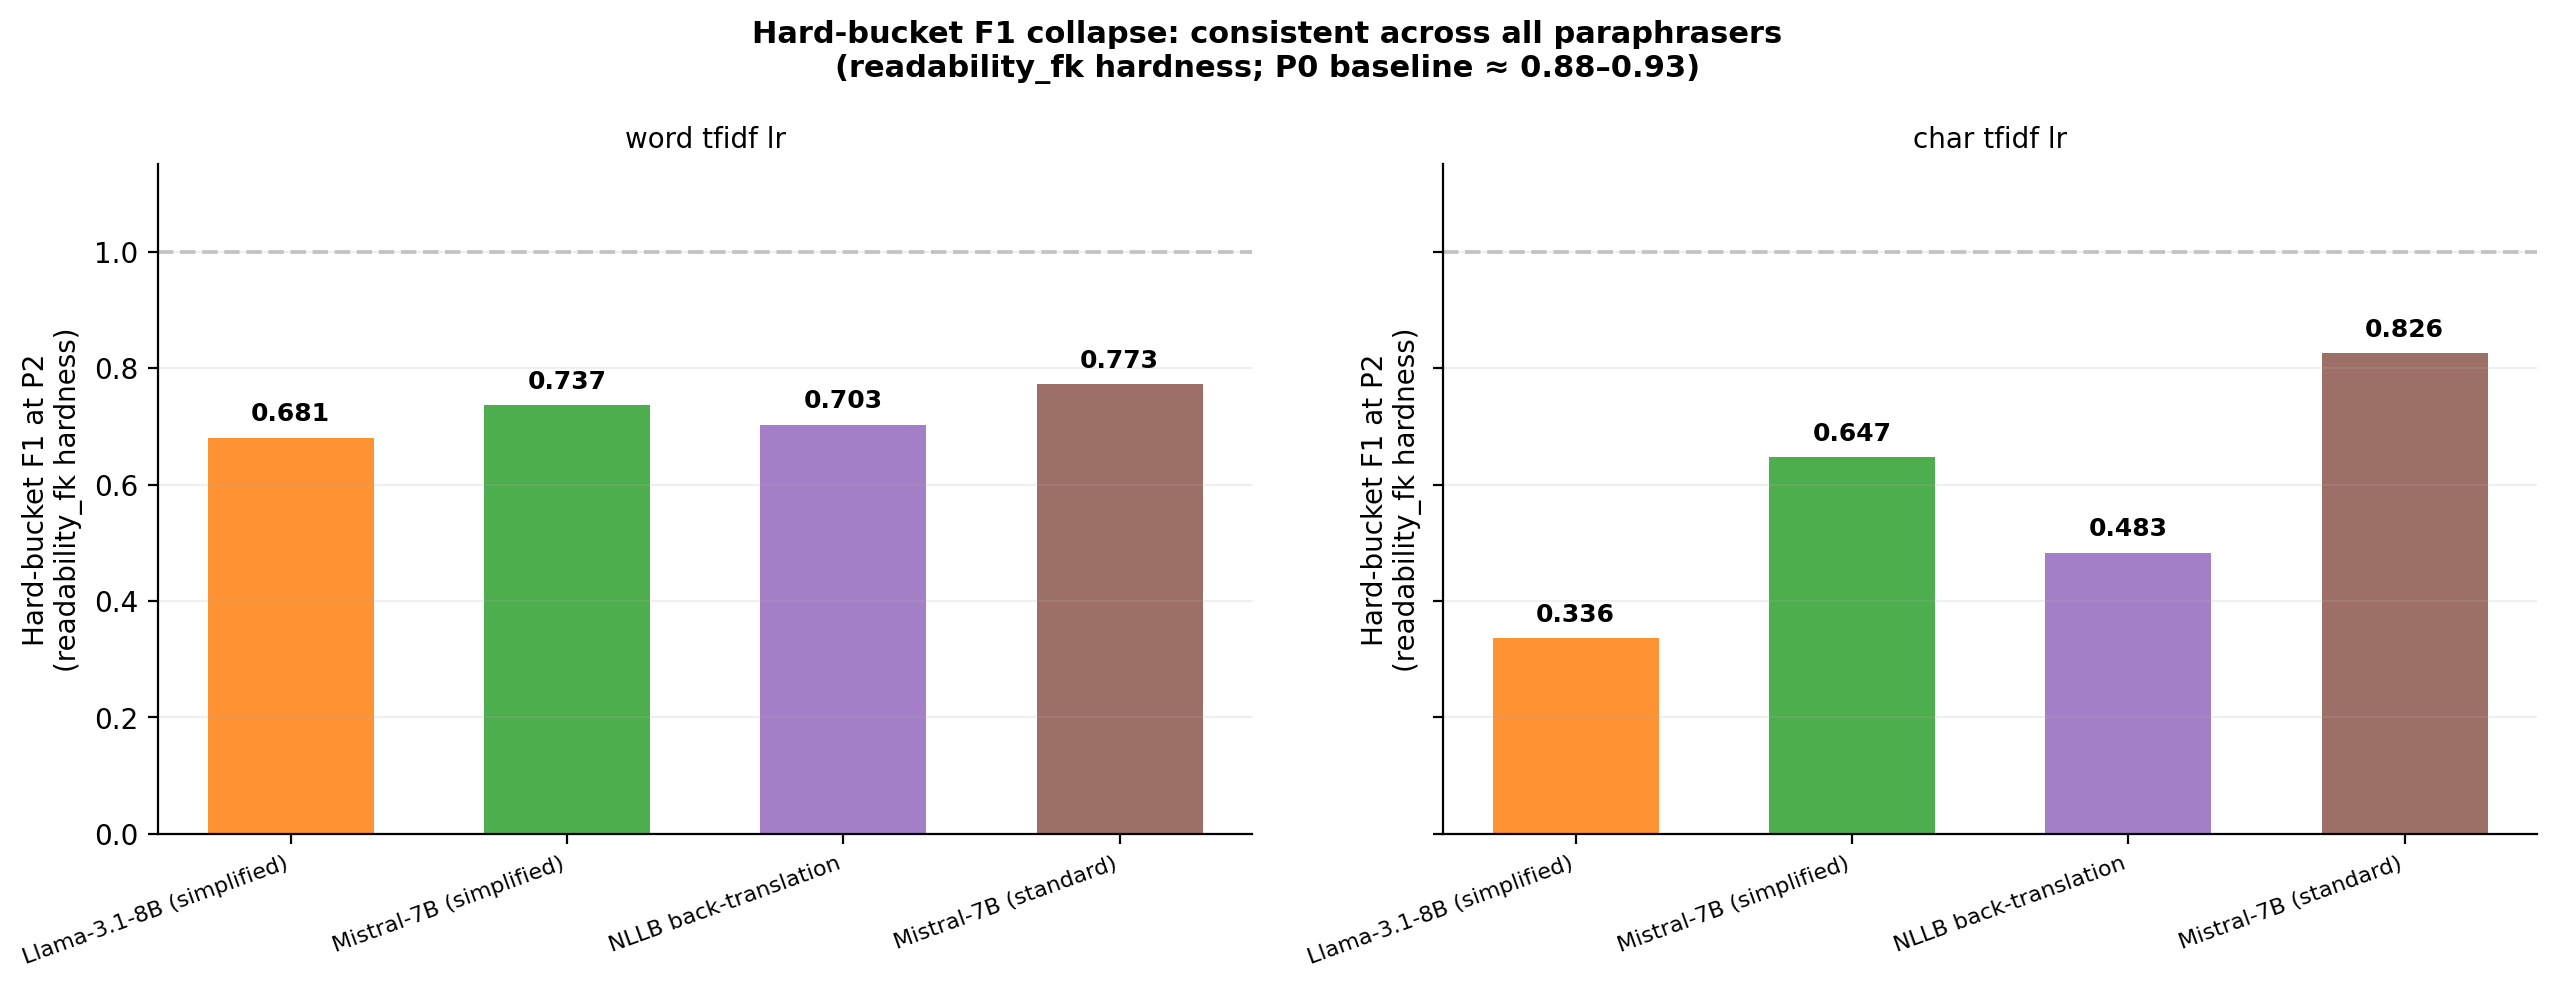
\includegraphics[width=0.85\linewidth]{fig17_three_paraphraser_comparison.png}
\caption{Hard-bucket $F_1$ at P2 across paraphrasers. Char-TF-IDF collapse is
consistent in direction across paraphraser families.}
\label{fig:fig17}
\end{figure}

That NLLB back-translation alone produces a meaningful Hard-bucket drop is
particularly informative: NLLB has no instruction tuning, no preference learning,
no LLM-style ``register.'' Its only effect is light lexical/syntactic
substitution. That this is sufficient to drop char-TF-IDF Hard $F_1$ by
\emph{0.44} tells us how surface-fragile the detector signal is.

% =============================================================================
\section{Mechanistic Analysis: Why Hard Examples Flip}
\label{sec:mechanism}

\subsection{Flip cases are entirely LLM-as-Human errors}

Define a \emph{flip} as a Hard-bucket example correctly classified at P0
but misclassified at P2 (simplified track). We count flips per detector:

\begin{itemize}
\item \textbf{char\_tfidf\_lr}: 16 flips out of 22 LLM examples in the Hard
bucket (\textbf{73\%}).
\textbf{All 16 are LLM samples} predicted as human at P2; \textbf{0 of the
12 human Hard examples flip.}
\item \textbf{word\_tfidf\_lr}: 8 flips out of 22 LLM Hard examples (\textbf{36\%}).
Again, all 8 are LLM-as-human; zero human flips.
\end{itemize}

The detectors do not become \emph{confused}—they become \emph{permissive}:
paraphrased LLM text drifts into the human region of feature space, while
human text stays put. This is a pure recall failure, not a precision failure,
and explains why aggregate accuracy can degrade severely while the false-positive
rate looks ``fine'' on average.

\FloatBarrier
\subsection{Top-feature SHAP attribution}
For a linear model on TF-IDF features the SHAP value of feature $i$ is exact
and has a simple form:
\begin{equation}
  \phi_i(x) \;=\; \beta_i \bigl(x_i - \bar{x}_i\bigr),
  \label{eq:shap}
\end{equation}
where $\beta_i$ is the logistic-regression coefficient, $x_i$ is the
feature value for input $x$, and $\bar{x}_i$ is the mean of that feature
over a background set (we use the training set). No sampling or
approximation is required. We compute mean $|\phi_i|$ across the
Hard-bucket flip cases at P0 and at P2, selecting the top-$K{=}20$
features by importance at each stage.

The top-5 char-TF-IDF features by mean $|\text{SHAP}|$ shift dramatically
between stages (Table~\ref{tab:shap_top}); the full top-20 is plotted in
Fig.~\ref{fig:fig20}.

\begin{table}[htbp]
\centering
\small
\begin{tabular}{c l l}
\toprule
\textbf{rank} & \textbf{P0 (correct)} & \textbf{P2-sim (wrong)} \\
\midrule
1 & \texttt{`\textvisiblespace var'}   & \texttt{`\textvisiblespace comp'} \\
2 & \texttt{`\textvisiblespace va'}    & \texttt{`comp'}                  \\
3 & \texttt{`ludin'}                   & \texttt{`omp'}                   \\
4 & \texttt{`cludi'}                   & \texttt{`\textvisiblespace it'}  \\
5 & \texttt{`ludi'}                    & \texttt{`can'}                   \\
\bottomrule
\end{tabular}
\caption{Top-5 char $n$-gram features by mean $|\text{SHAP}|$ on the same 16
Hard-bucket flip cases, before and after paraphrasing.
P0 features are fragments of formal/academic words (\emph{variables, including});
P2-simplified features are generic, short, everyday $n$-grams.
The visible-space character (\textvisiblespace) denotes a word-boundary space
in the \texttt{char\_wb} analyser.}
\label{tab:shap_top}
\end{table}

\begin{figure}[htbp]
\centering
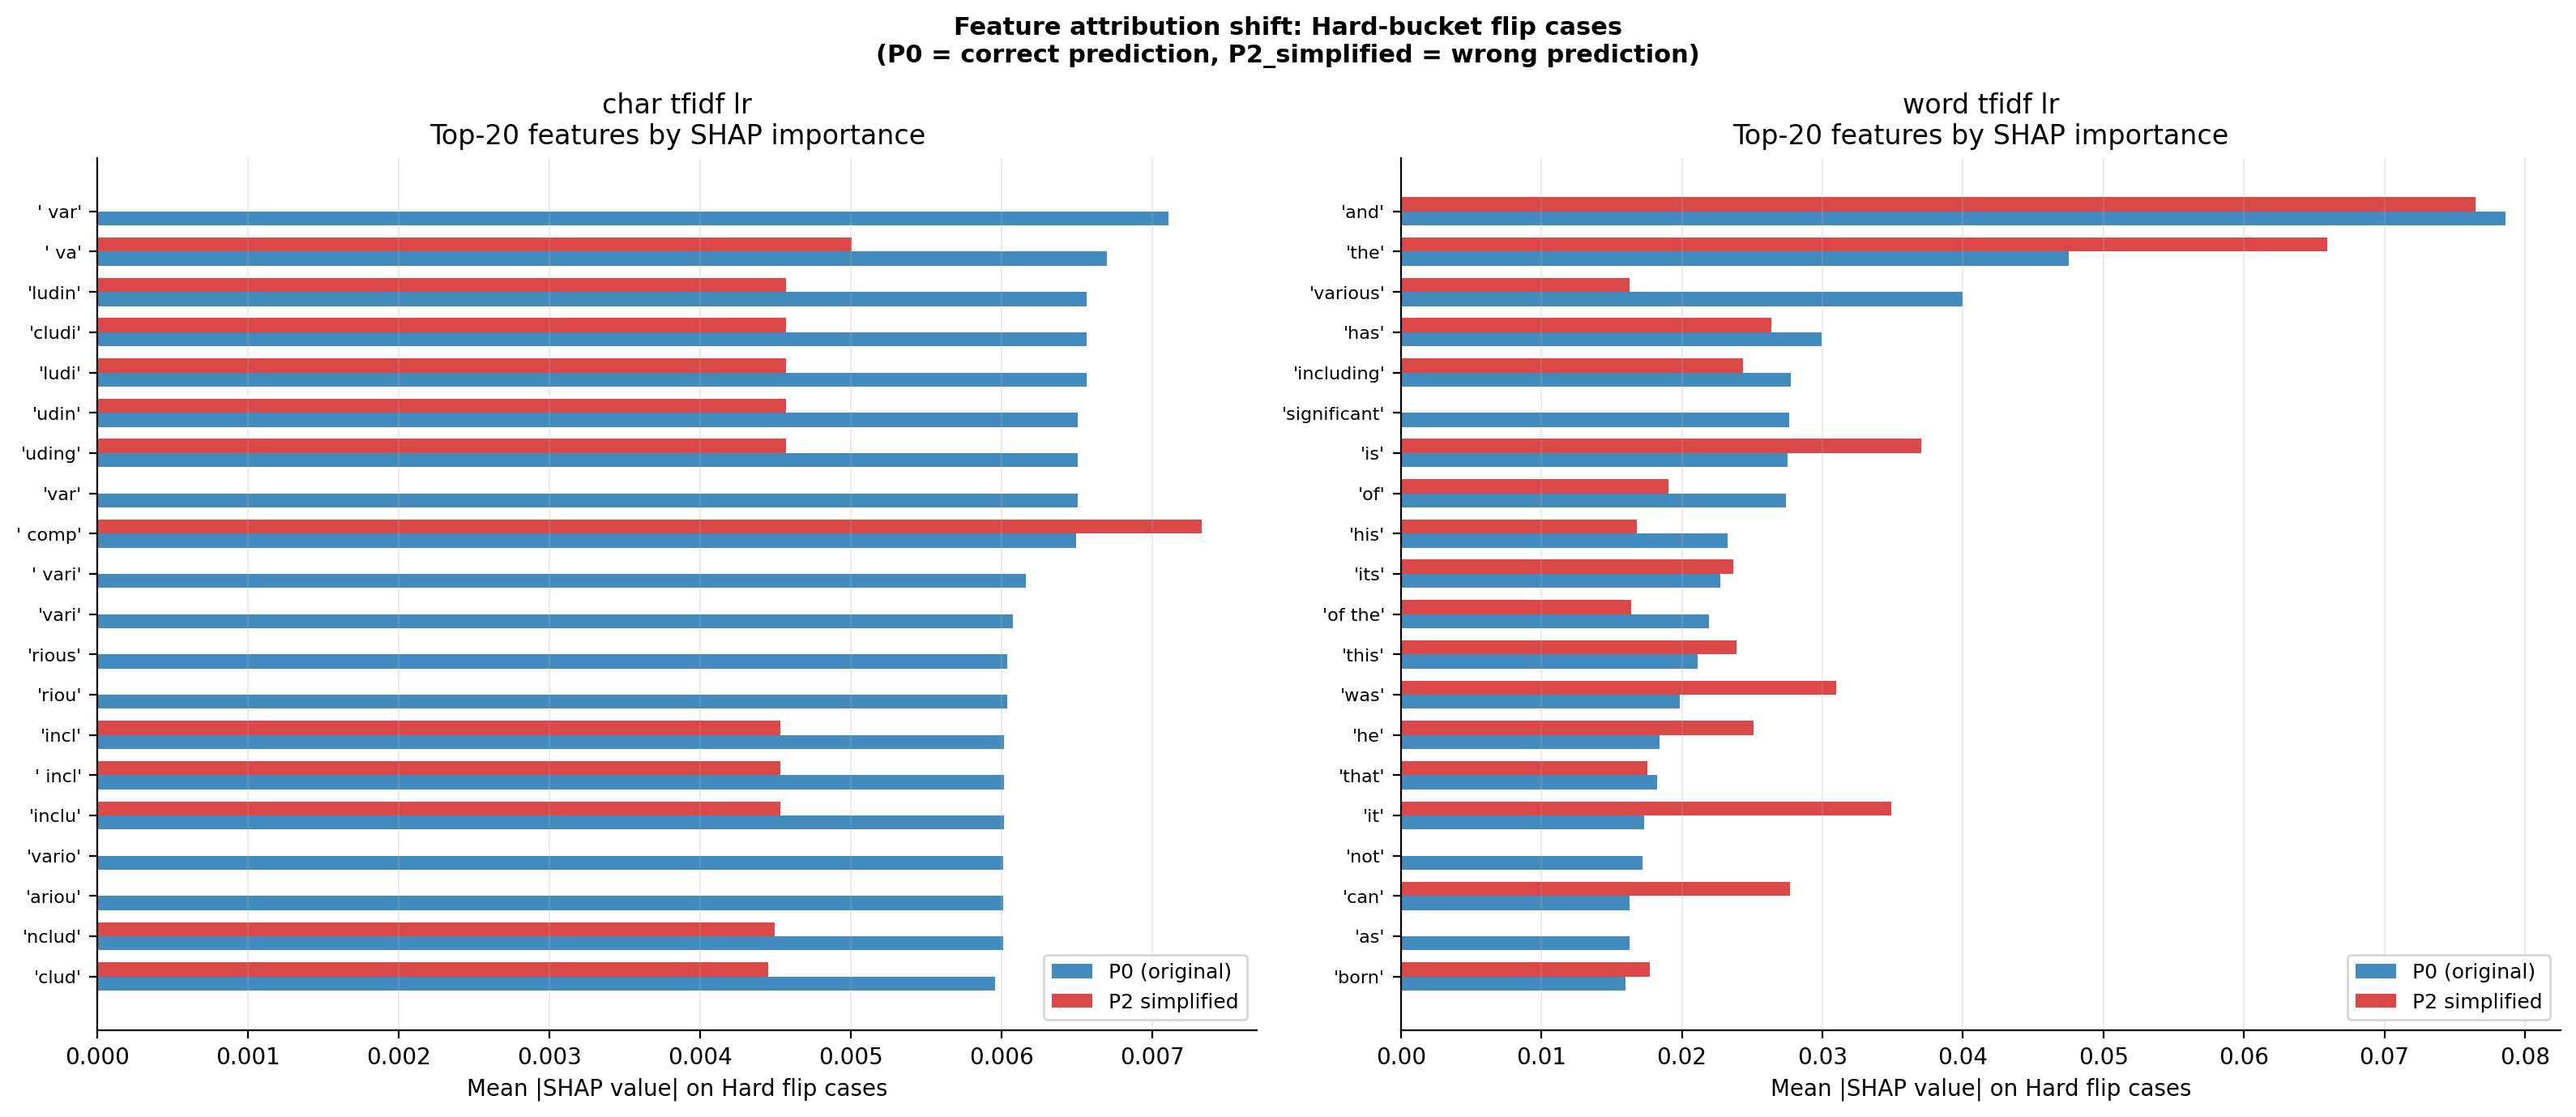
\includegraphics[width=0.85\linewidth]{fig20_shap_top_features.png}
\caption{Top-20 features by mean $|\text{SHAP}|$ on Hard-bucket flip cases,
P0 vs P2-simplified. The feature set rotates almost entirely.}
\label{fig:fig20}
\end{figure}

\FloatBarrier
\subsection{Feature survival}
A direct way to test the ``surface-fragility'' hypothesis is to count
how many of the detector's top-20 features (ranked by $|\beta|$ on the
training set) survive into the paraphrased text. ``Survives'' means the
$n$-gram still has a non-zero TF-IDF weight in the paraphrased version of the
same paragraph (Table~\ref{tab:survival}, Fig.~\ref{fig:fig21}).

\begin{table}[htbp]
\centering
\small
\begin{tabular}{lc}
\toprule
\textbf{Detector} & \textbf{Top-20 feature survival rate (P0 $\to$ P2-sim)} \\
\midrule
char\_tfidf\_lr & \textbf{13.1\%} (LLM flip cases) \\
word\_tfidf\_lr & 26.2\% (LLM flip cases) \\
\bottomrule
\end{tabular}
\caption{Fraction of the top-20 detector cues that survive paraphrasing in
Hard-bucket flip cases. Char-TF-IDF loses 87\% of its top cues.}
\label{tab:survival}
\end{table}

\begin{figure}[htbp]
\centering
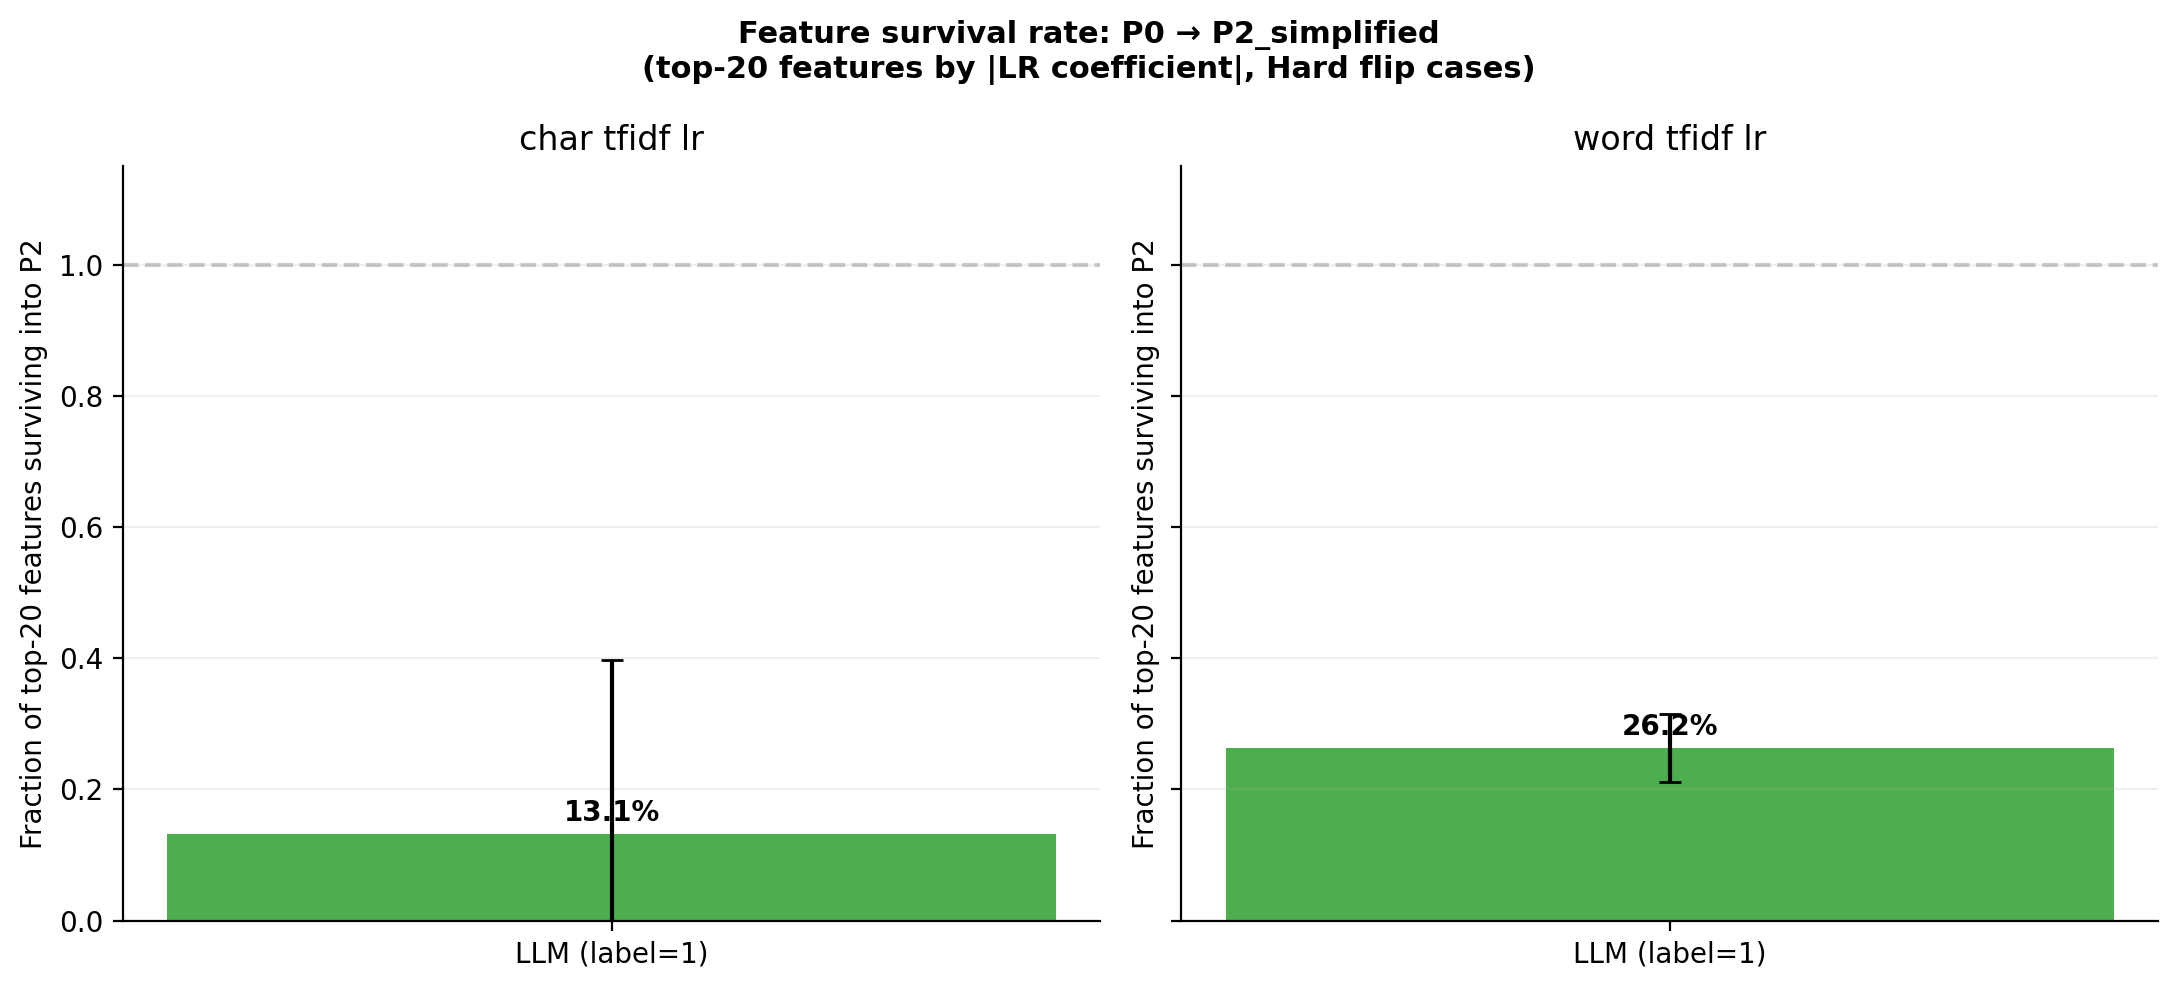
\includegraphics[width=0.55\linewidth]{fig21_feature_survival.png}
\caption{Fraction of top-20 features by $|\beta|$ surviving paraphrasing in
flip cases. Only LLM-labelled rows are shown because, as noted above, no
human rows flip.}
\label{fig:fig21}
\end{figure}

\FloatBarrier
\subsection{Vocabulary homogenisation}
Why do the features disappear? Simplified paraphrasing shrinks the mean word
length for both human and LLM texts, collapsing them onto the same lexical
register (Table~\ref{tab:wlen}, Fig.~\ref{fig:fig22}):

\begin{table}[H]
\centering
\small
\begin{tabular}{lccc}
\toprule
\textbf{Group} & \textbf{P0} & \textbf{P1-sim} & \textbf{P2-sim} \\
\midrule
Human (Hard bucket) & 5.21 & 4.76 & 4.76 \\
LLM   (Hard bucket) & 5.36 & 4.74 & 4.71 \\
\bottomrule
\end{tabular}
\caption{Mean word length (characters) in the Hard bucket across paraphrase
rounds. The LLM's vocabulary is initially more formal (5.36 vs 5.21); after
one round of simplified paraphrasing the two groups are indistinguishable.
The character $n$-gram signature the detector relies on is built into this gap.}
\label{tab:wlen}
\end{table}

\begin{figure}[H]
\centering
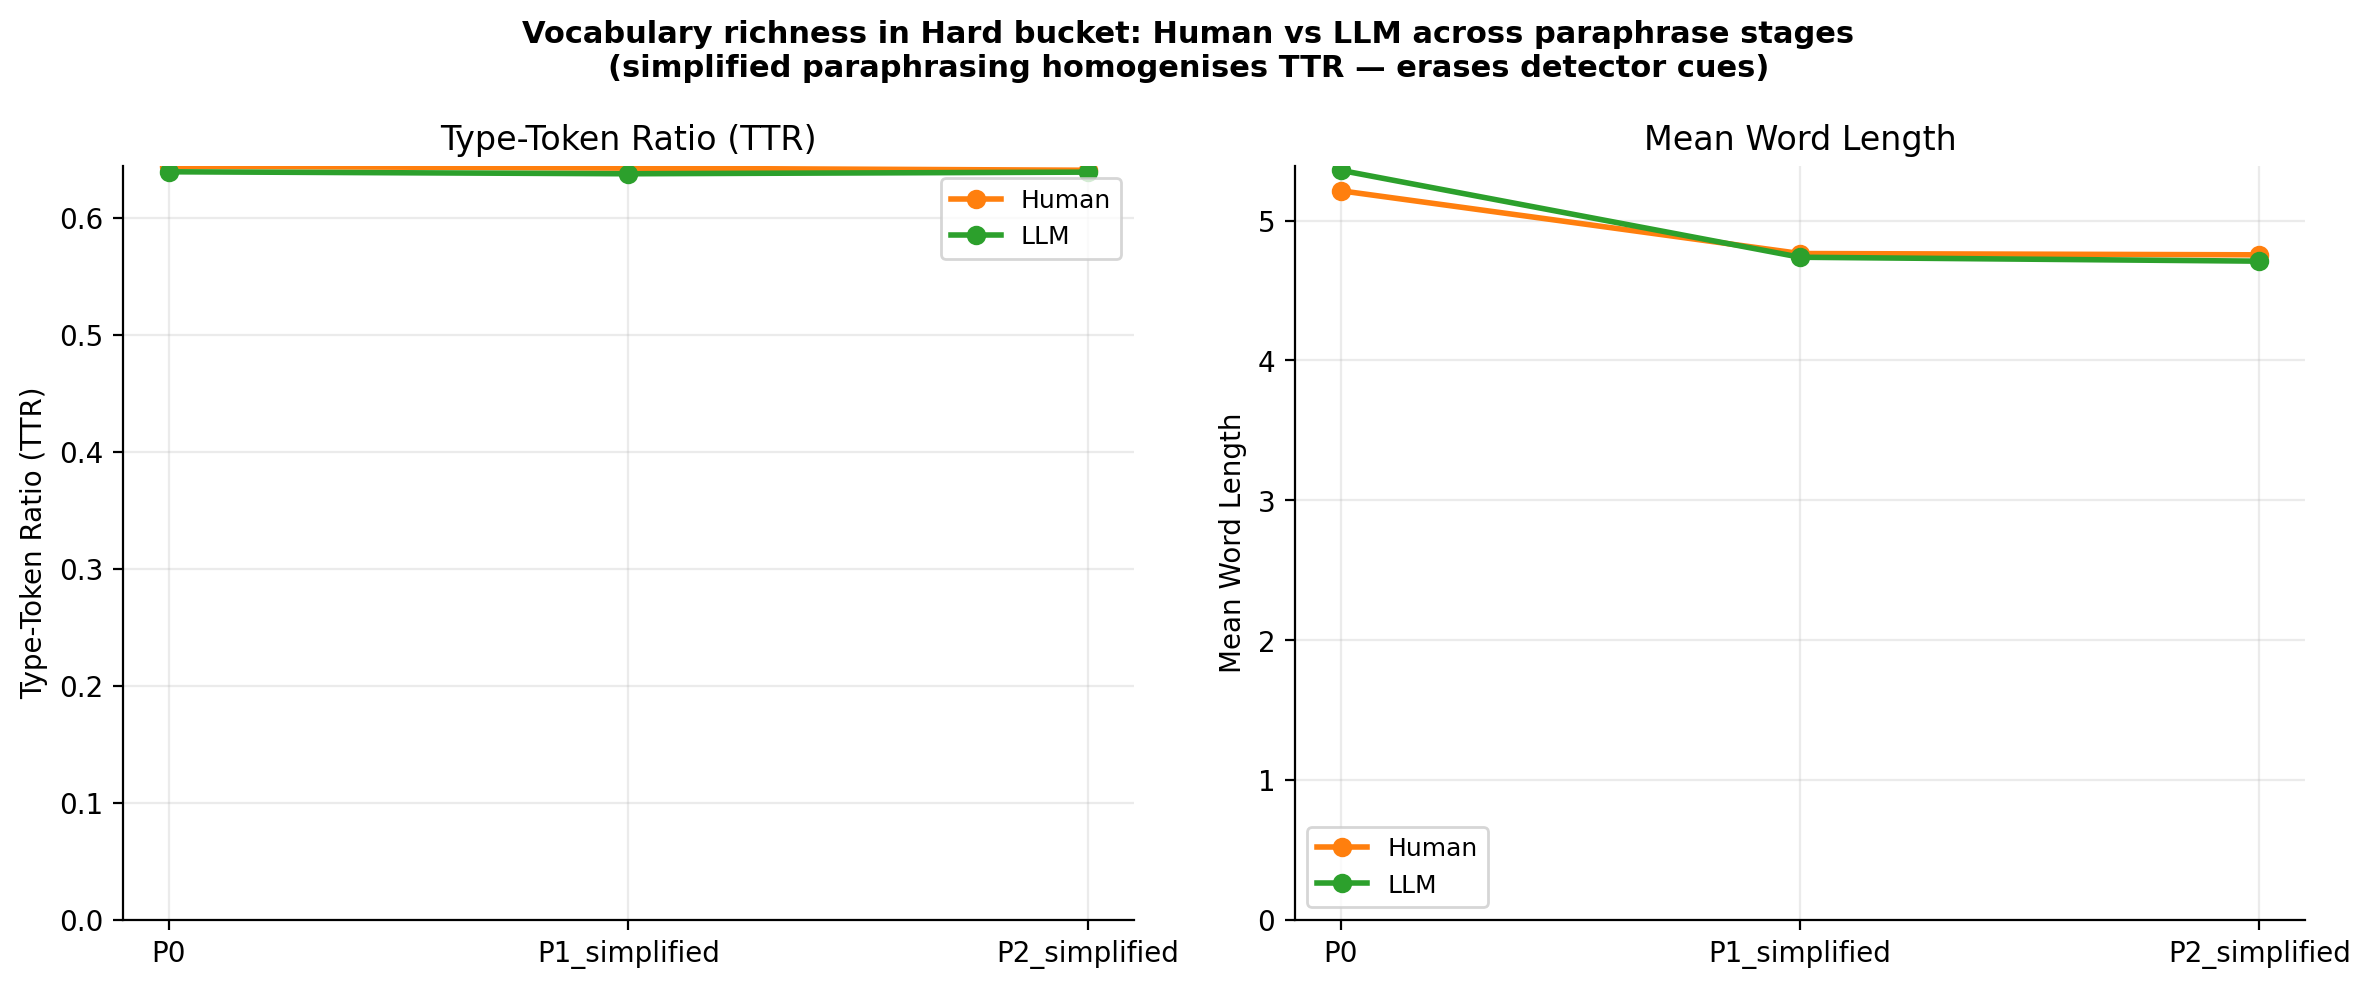
\includegraphics[width=0.82\linewidth]{fig22_vocab_drift.png}
\caption{Vocabulary drift on the Hard bucket. Type-token ratio is roughly
constant; mean word length drops for both groups, with the LLM dropping
further, eliminating the formal-register gap.}
\label{fig:fig22}
\end{figure}

We read this as a clean mechanistic story:
\textbf{the char-TF-IDF detector exploits a formal-register gap between
LLM and human writing at the character level; simplified paraphrasing erases
that gap; the detector loses its cues; LLM texts in the Hard bucket cross the
decision boundary into the human region.}

\FloatBarrier
\subsection{A concrete flip example}
\label{sec:concrete_flip}

To make the mechanism tangible, Table~\ref{tab:concrete_example} shows one
representative Hard-bucket flip case in full: an LLM-generated paragraph
about botany that the char-TF-IDF detector identifies as LLM at P0
(probability 0.858), correctly, then fails to identify at P2 (probability
0.410), incorrectly. The two-round simplified paraphrase reduces mean word
length from 6.28 to 4.81 characters (a 23\% drop) and replaces academic
vocabulary—\emph{encompasses, disciplines, morphology, biochemistry,
systematics, photosynthesis}—with everyday alternatives—\emph{looks at,
make babies, tiny building blocks}. The semantic content is preserved
but the character-$n$-gram signature is destroyed.

\begin{table}[H]
\centering
\small
\begin{tabular}{p{0.95\linewidth}}
\toprule
\textbf{P0 (Llama-3.1-8B original).} char-TF-IDF
$P(\mathrm{LLM})=\mathbf{0.858}$; mean word length 6.28; 151 words. \\
\midrule
\emph{Botany is the scientific study of plants, including their structure,
growth, development, reproduction, metabolism, evolution, and classification.
It encompasses a wide range of disciplines, from plant anatomy and morphology
to physiology, biochemistry, genetics, ecology, and systematics. Botanists
investigate various aspects of plant biology, such as photosynthesis,
respiration, nutrient uptake, and response to environmental stimuli. They
also study the diversity of plant species, including their classification,
distribution, and interactions with other organisms in ecosystems\ldots} \\
\midrule
\textbf{P2 (after 2 rounds of simplified paraphrasing).} char-TF-IDF
$P(\mathrm{LLM})=\mathbf{0.410}$; mean word length 4.81; 113 words. \\
\midrule
\emph{The study of plants is called botany. It's a science that looks at
how plants grow, develop, and make babies. Botany also studies how plants
make their own food and how they react to their surroundings. Botanists
examine the different parts of plants, like their tiny building blocks,
and how they work together. They also study the many different types of
plants and where they can be found\ldots} \\
\bottomrule
\end{tabular}
\caption{One Hard-bucket flip case in full. The 0.448 drop in
$P(\mathrm{LLM})$ co-occurs with a 23\% drop in mean word length and a
wholesale lexical substitution of formal academic terms for everyday
language. The semantic content (what botany is, what botanists do) is
preserved; the character-level register signal that the detector relied
on is not.}
\label{tab:concrete_example}
\end{table}

\FloatBarrier
\subsection{The signal is preserved in embeddings — only surface features collapse}
\label{sec:embedding_projection}

The flip example above suggests semantic content survives paraphrasing while
the surface signature does not. We verify this directly with embedding
analysis. For every Hard-bucket text at P0, P1-simplified, and P2-simplified
we compute an SBERT representation (\texttt{all-mpnet-base-v2}, 768-D) and
project the joint set into 2-D with UMAP (Fig.~\ref{fig:umap_hard}).

In the original 768-D space, the cosine distance between Human and LLM
centroids in the Hard bucket is $0.605$ at P0, $0.511$ at P1, and
$0.479$ at P2 — a 21\% reduction.
Meanwhile, in the same examples, char-TF-IDF Hard $F_1$ drops 64\%
(0.923 $\to$ 0.336) and RoBERTa Hard $F_1$ drops only 8\% (1.000 $\to$ 0.920).

\begin{figure}[htbp]
\centering
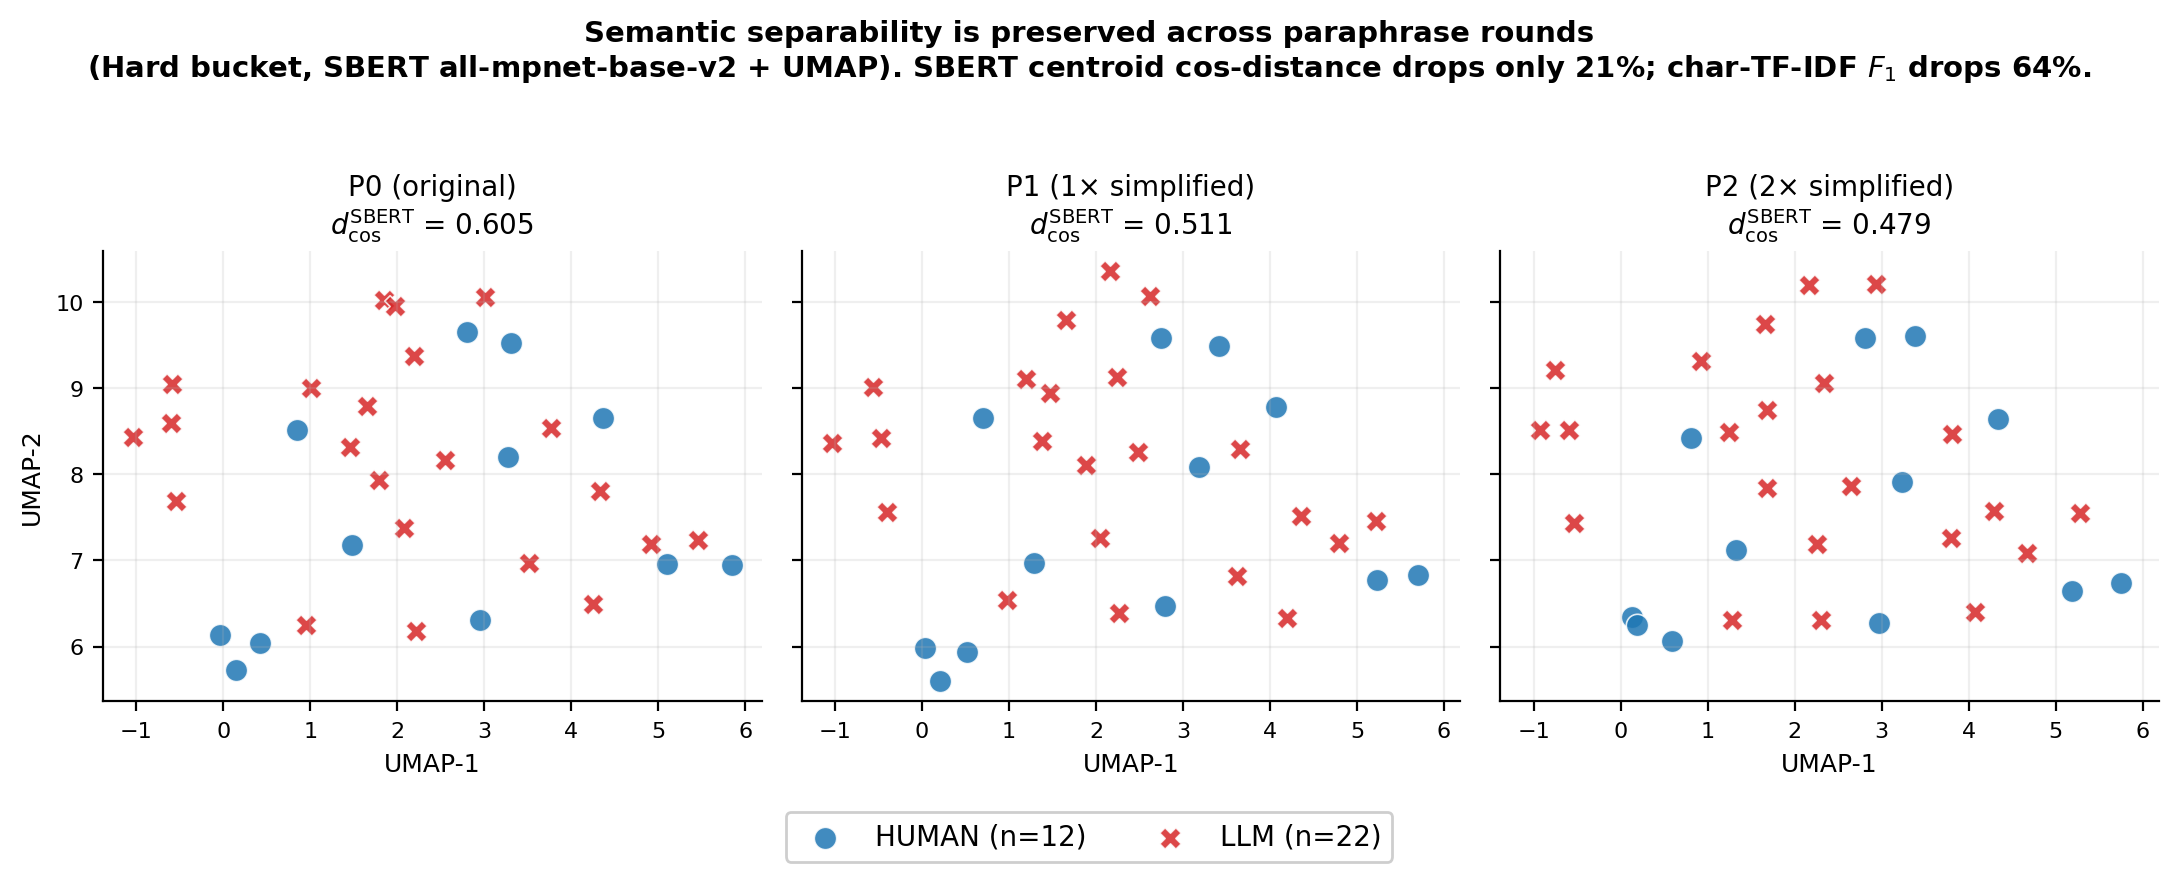
\includegraphics[width=0.95\linewidth]{fig23_umap_hard_bucket.png}
\caption{UMAP projection of SBERT embeddings (Hard bucket, 12 Human / 22
LLM). Class separability erodes only modestly across paraphrase rounds: the
SBERT centroid cosine-distance shrinks by 21\%, far less than char-TF-IDF's
64\% $F_1$ drop on the same examples. The signal char-TF-IDF loses is still
present in embeddings — which is why RoBERTa-base remains robust on the same
texts.}
\label{fig:umap_hard}
\end{figure}

This is the missing piece that ties \S\ref{sec:detector_family} to
\S\ref{sec:mechanism}: \textbf{the simplified-paraphrase attack does not
destroy the information needed to distinguish Human from LLM — it destroys
only the specific surface-feature encoding that char-TF-IDF relies on}.
Detectors with access to deeper representations (RoBERTa) keep most of their
discriminative power; detectors restricted to character $n$-grams do not.

% =============================================================================
\section{Calibration Under Distribution Shift}
\label{sec:calibration}

We also asked whether confidences output by the detectors remain usable
across paraphrase rounds. Concretely: if we fit a temperature on the
validation set (standard ECE calibration), does it carry over to the
paraphrased test splits? (Table~\ref{tab:calibration},
Fig.~\ref{fig:fig18}.)

\begin{table}[htbp]
\centering
\small
\begin{tabular}{lcccc}
\toprule
\textbf{Detector} & \textbf{$T_{\rm opt}$} & \textbf{ECE P0 (after $T$)} & \textbf{ECE P2-sim (after $T$)} & $\Delta$ \\
\midrule
word\_tfidf\_lr  & 0.18 & 0.32 & 0.36 & $+0.13$ \\
char\_tfidf\_lr  & 0.16 & 0.36 & 0.40 & $+0.12$ \\
roberta\_base    & --   & 0.38 & 0.37 & $-0.00$ \\
\bottomrule
\end{tabular}
\caption{Temperature scaling fit on validation (TF-IDF only) and applied to
test splits. $T_{\rm opt} \!\ll\! 1$ implies the TF-IDF detectors are
\emph{overconfident}. Calibration is acceptable at P0 but degrades sharply at
P2-simplified—the same place $F_1$ collapses. RoBERTa is poorly calibrated
everywhere but its miscalibration is stable.}
\label{tab:calibration}
\end{table}

\begin{figure}[htbp]
\centering
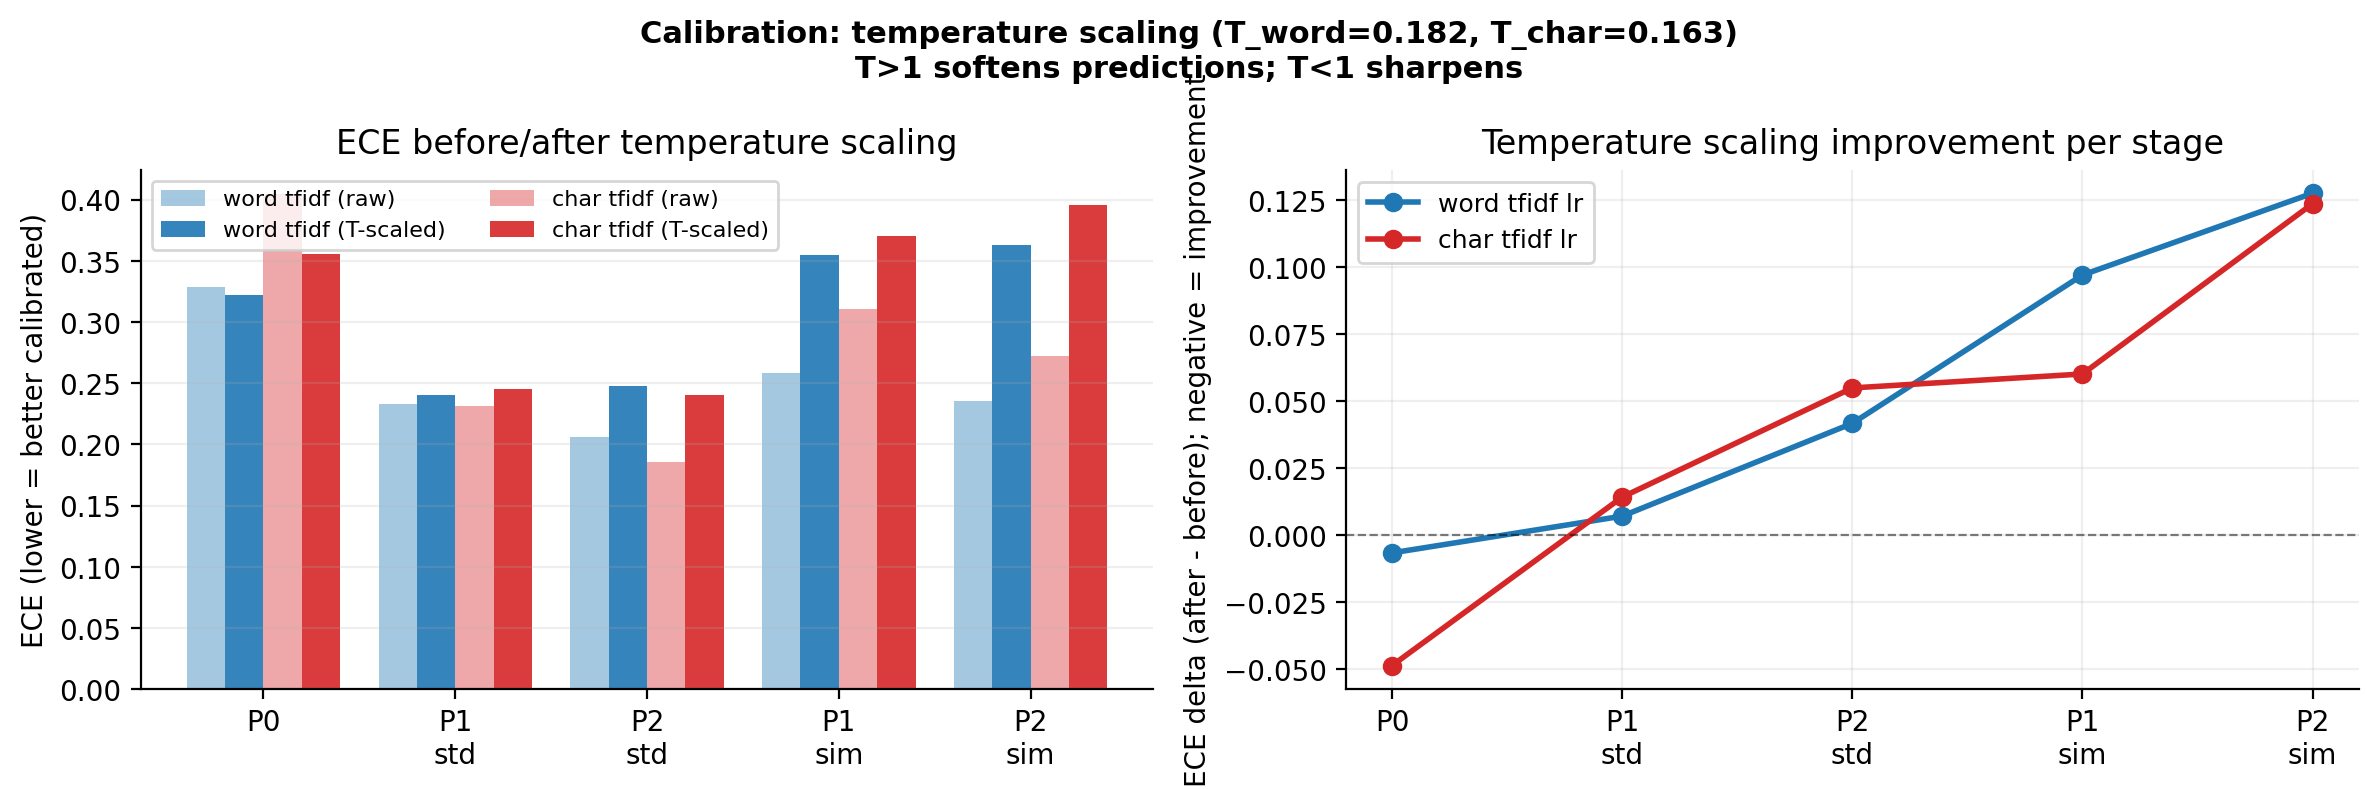
\includegraphics[width=0.82\linewidth]{fig18_temperature_scaling.png}
\caption{Reliability curves before and after temperature scaling.
TF-IDF detectors are massively overconfident at P0; $T$-scaling fixes that;
under paraphrasing the same $T$ now over-corrects.}
\label{fig:fig18}
\end{figure}

The practical implication is that
\emph{validation-fit temperature is not a substitute for retraining}
under paraphrase-style distribution shift, even when the underlying
classifier $F_1$ is still well above chance.

% =============================================================================
\section{Discussion}

\paragraph{Why does char-TF-IDF fail where RoBERTa does not?}
Our results favour a clean explanation:
RoBERTa's representations encode meaning, and meaning is precisely what the
paraphraser prompts are instructed to preserve. Char-TF-IDF representations
encode surface form, which is precisely what the simplified prompt is
instructed to change. Word-TF-IDF sits in between. The detector-family
asymmetry is therefore not a curiosity—it is a direct consequence of which
aspects of text each family represents.

\paragraph{Why is Mistral-7B's collapse milder than Llama's?}
Under the simplified prompt, Mistral-7B produces a Hard-bucket char-TF-IDF
$F_1$ of 0.647 vs.\ Llama's 0.336—a gap of 0.31. The most plausible
explanation is \emph{prompt-following fidelity}: Llama-3.1-8B (an
instruction-tuned model) adheres more aggressively to the ``simple
vocabulary'' constraint, erasing the formal-register character signal more
thoroughly than Mistral does. This suggests that as paraphraser instruction-following
improves, the surface-feature collapse will worsen—making RoBERTa-class
detectors increasingly necessary.

\paragraph{What would be a robust feature?}
If our reading is right, a robust detector must encode aspects of text that
\emph{instruction-tuned LLMs cannot freely rewrite}. Embedding-space
distances and discourse-level coherence patterns are plausible candidates.
Surface character $n$-grams are not.

\paragraph{Should detectors report Hard-bucket $F_1$?}
We argue yes. Reporting aggregate $F_1$ on a test set whose Easy:Medium:Hard
balance is unspecified is uninformative for downstream deployment. A simple,
text-only stratification (e.g.\ readability tertile on P0 text) is essentially
free and gives a much clearer picture of where a system breaks.

\paragraph{Limitations.}
\textbf{(i) Scale.} Our test set is 100 paragraphs. We compensate with paired
multi-seed bootstrap intervals and exhaustive paraphraser ablation, but
larger test sets would tighten the CIs.
\textbf{(ii) Generator scope.} Our LLM-side training data come from a single
generator (Llama-3.1-8B). Cross-generator evaluation (e.g.\ training on
Llama and testing on GPT-4 outputs) is left to future work.
\textbf{(iii) Watermarking.} We do not study watermarked text. Watermark-based
detectors may have different robustness profiles under
paraphrase~\citep{krishna2023paraphrasing}.

% =============================================================================
\section{Conclusion}

Robustness of LLM-text detection is heterogeneous, and the heterogeneity is
predictable. The Hard tertile of a readability-stratified test set
absorbs nearly all of the degradation under simplified paraphrasing.
The collapse reproduces across three paraphrasers from distinct families,
is detector-family-specific (catastrophic for character $n$-grams, mild for
transformer encoders), is asymmetric (LLM-as-human, not human-as-LLM),
and is mechanistically explained by feature survival and vocabulary
homogenisation in the Hard bucket.

We hope this work motivates two practical changes in robustness reporting:
\emph{stratify by hardness}, and \emph{vary the paraphraser family}.

% =============================================================================
\section*{Reproducibility}
All code, data splits, paraphrased corpora, model weights, evaluation CSVs,
and figures used in this paper are released at
\url{https://github.com/razon1494/Analysis-of-Human-vs.-LLM-Generated-Text}.
The repository includes per-experiment driver scripts under
\texttt{src/experiments/} and a deterministic split file under
\texttt{data/splits/}.

% =============================================================================
\bibliographystyle{plainnat}
\begin{thebibliography}{99}

\bibitem[Gehrmann et~al.(2019)]{gehrmann2019gltr}
Gehrmann, S., Strobelt, H., \& Rush, A.~M. (2019).
\newblock GLTR: Statistical Detection and Visualization of Generated Text.
\newblock \emph{ACL System Demonstrations}.

\bibitem[Guo et~al.(2023)]{guo2023gpt}
Guo, B., Zhang, X., Wang, Z., et~al.\ (2023).
\newblock How Close is ChatGPT to Human Experts? Comparison Corpus, Evaluation, and Detection.
\newblock \emph{arXiv:2301.07597}.

\bibitem[Kirchenbauer et~al.(2023)]{kirchenbauer2023watermark}
Kirchenbauer, J., Geiping, J., Wen, Y., et~al.\ (2023).
\newblock A Watermark for Large Language Models.
\newblock \emph{ICML}.

\bibitem[Krishna et~al.(2023)]{krishna2023paraphrasing}
Krishna, K., Song, Y., Karpinska, M., et~al.\ (2023).
\newblock Paraphrasing evades detectors of AI-generated text, but retrieval is an effective defense.
\newblock \emph{NeurIPS}.

\bibitem[Mitchell et~al.(2023)]{mitchell2023detectgpt}
Mitchell, E., Lee, Y., Khazatsky, A., et~al.\ (2023).
\newblock DetectGPT: Zero-Shot Machine-Generated Text Detection using Probability Curvature.
\newblock \emph{ICML}.

\bibitem[NLLB Team(2022)]{nllb2022}
NLLB Team (2022).
\newblock No Language Left Behind: Scaling Human-Centered Machine Translation.
\newblock \emph{arXiv:2207.04672}.

\bibitem[Rajpurkar et~al.(2018)]{rajpurkar2018know}
Rajpurkar, P., Jia, R., \& Liang, P. (2018).
\newblock Know What You Don't Know: Unanswerable Questions for SQuAD.
\newblock \emph{ACL}.

\bibitem[Sadasivan et~al.(2023)]{sadasivan2023can}
Sadasivan, V.~S., Kumar, A., Balasubramanian, S., et~al.\ (2023).
\newblock Can AI-Generated Text be Reliably Detected?
\newblock \emph{arXiv:2303.11156}.

\bibitem[Taori et~al.(2020)]{taori2020measuring}
Taori, R., Dave, A., Shankar, V., et~al.\ (2020).
\newblock Measuring Robustness to Natural Distribution Shifts in Image Classification.
\newblock \emph{NeurIPS}.

\end{thebibliography}

\end{document}

% =============================================================================
%  HOW TO SWITCH TO ACL 2-COLUMN FORMAT FOR VENUE SUBMISSION (TrustNLP, EMNLP)
% =============================================================================
%
%  Replace the preamble block at the top of this file with:
%
%    \documentclass[11pt]{article}
%    \usepackage[T1]{fontenc}
%    \usepackage[utf8]{inputenc}
%    \usepackage{acl}                 % requires acl.sty in project
%    \usepackage{times}
%    \usepackage{latexsym}
%    \usepackage{microtype}
%    \usepackage{amsmath,amssymb}
%    \usepackage{booktabs}
%    \usepackage{multirow}
%    \usepackage{graphicx}
%    \usepackage{xcolor}
%    \usepackage{url}
%    \usepackage{hyperref}
%    \usepackage[section]{placeins}
%    \usepackage{subcaption}
%    \usepackage{float}
%    \graphicspath{{figures/}{../figures/}}
%    \title{Hardness-Aware Robustness of LLM-Text Detection ...}
%    \author{Mohammad Arifur Rahman \\
%            Anderson University \\
%            \texttt{rahman.arif.cse@gmail.com}}
%
%  And change \bibliographystyle{plainnat} to \bibliographystyle{acl_natbib}.
%  For anonymous double-blind review, use \usepackage[review]{acl} instead.
% =============================================================================
